\documentclass[onecolumn, draftclsnofoot,10pt, compsoc]{IEEEtran}
\usepackage{url}
\usepackage{setspace}
\usepackage{graphicx}
\usepackage{epstopdf}
\epstopdfsetup{update} % only regenerate pdf files when eps file is newer
\usepackage[utf8]{inputenc}
\usepackage[english]{babel}
\usepackage{indentfirst}
\usepackage{geometry}
\usepackage{color}
\usepackage{tikz}
\usepackage{rotating}
\usepackage{pgfgantt}
\usepackage{xcolor}
\geometry{textheight=9.5in, textwidth=7in}


\newganttchartelement{orangebar}{
    orangebar/.style={
        inner sep=0pt,
        draw=red!66!black,
        very thick,
        top color=white,
        bottom color=orange!80
    },
    orangebar label font=\slshape,
    orangebar left shift=.1,
    orangebar right shift=-.1
}

\newganttchartelement{bluebar}{
    bluebar/.style={
        inner sep=0pt,
        draw=purple!44!black,
        very thick,
        top color=white,
        bottom color=blue!80
    },
    bluebar label font=\slshape,
    bluebar left shift=.1,
    bluebar right shift=-.1
}


% 1. Fill in these details
\def \CapstoneTeamName{		MAV CHALLENGE}
\def \CapstoneTeamNumber{		32}
\def \GroupMemberOne{			Justin Sherburne}
\def \GroupMemberTwo{			Kaiyuan Fan}
\def \GroupMemberThree{			Yingshi Huang}
\def \CapstoneProjectName{		AHS Micro-Air Vehicle Challenge}
%\def \CapstoneSponsorCompany{	Columbia Helicopters}
\def \CapstoneSponsorPerson{		Nancy Squires, Ph.D.}

% 2. Uncomment the appropriate line below so that the document type works
\def \DocType{		%Problem Statement
				%Requirements Document
				%Technology Review
				Final Report
				%Progress Report
				}
			
\newcommand{\NameSigPair}[1]{\par
\makebox[2.75in][r]{#1} \hfil 	\makebox[3.25in]{\makebox[2.25in]{\hrulefill} \hfill		\makebox[.75in]{\hrulefill}}
\par\vspace{-12pt} \textit{\tiny\noindent
\makebox[2.75in]{} \hfil		\makebox[3.25in]{\makebox[2.25in][r]{Signature} \hfill	\makebox[.75in][r]{Date}}}}
% 3. If the document is not to be signed, uncomment the RENEWcommand below
\renewcommand{\NameSigPair}[1]{#1}

%%%%%%%%%%%%%%%%%%%%%%%%%%%%%%%%%%%%%%%
\begin{document}
\begin{titlepage}
    \pagenumbering{gobble}
    \begin{singlespace}
    	
\includegraphics[height=4cm]{coe_v_spot1}
        \hfill 
        % 4. If you have a logo, use this includegraphics command to put it on the coversheet.
        %\includegraphics[height=4cm]{CompanyLogo}   
        \par\vspace{.2in}
        \centering
        \scshape{
            \huge CS Capstone \DocType \par
            {\large\today}\par
            \vspace{8pt}
            \textbf{\Huge\CapstoneProjectName}\par
			\vspace{1.5in}
            {\large Prepared for}\par
            % \Huge \CapstoneSponsorCompany\par
            % \vspace{5pt}
            {\Large\NameSigPair{\CapstoneSponsorPerson}\par}
			\vspace{3pt}
            {\large Prepared by }\par
            Group\CapstoneTeamNumber\par
            % 5. comment out the line below this one if you do not wish to name your team
            \CapstoneTeamName\par 
            \vspace{8pt}
            {\Large
                \NameSigPair{\GroupMemberOne}\par
                \NameSigPair{\GroupMemberTwo}\par
                \NameSigPair{\GroupMemberThree}\par
            }
            \vspace{.5in}
        }
        \begin{abstract}
        The purpose of this document is to compile all documentation from this project into a single source. This is a culmination of the work contributed by the computer science team for the Micro Air-Vehicle challenge project. We will provide in-depth summaries regarding weekly activities, research, and design attributes for this project. Design choices, key project components, and installation instructions will also be covered in this report.
        
        \end{abstract}     
    \end{singlespace}
\end{titlepage}
\newpage
\pagenumbering{arabic}
\tableofcontents
% 7. uncomment this (if applicable). Consider adding a page break.
\listoffigures
%\listoftables
\clearpage


\section*{Revision History}

\begin{center}
    \begin{tabular}{|c|c|c|c|}
        \hline
		Name & Date & Reason For Changes & Version\\
        \hline
		Design Document & Nov 29, 2017 & Initial Creation & 1.0\\
		\hline 
    \end{tabular}
\end{center}



\section{Introduction}


\subsection{Project Overview}

This project has been proposed by Dr. Nancy Squires. Dr. Squires sponsors a number of collaboratory projects within the College of Engineering, with this being the newest project under her guidance. Dr. Squires served as the supervisor and sponsor for this project. All project planning, design, and implementation was left to the project team members. The goal of this project is to compete in the annual AHS Micro-Air Vehicle challenge\cite{r2} and to create additional venues for Oregon State University to represent itself in professional competitions.  


\subsection{The Project}

The Micro-Air Vehicle challenge\cite{r2} is an annual collegiate competition hosted by The American Helicopter Society. The competition is conducted by the AHS International Unmanned VTOL Aircraft and Rotor craft Committee. Competitors are tasked with building a vehicle capable of steady-state hovering, avoiding obstacles, and recognizing a drop-off point. This vehicle may compete in either a manual or autonomous flight category. The aircraft is remotely controlled and will have the ability to deliver packages to a specified location.

\subsection{Importance}

The purpose of this project is to represent Oregon State University in a professional competition. This is OSU's fist attempt at this competition, and we want to go with the best possible aircraft. In the event that the aircraft cannot meet all of the competition requirements we will not attend the competition and pass on knowledge to next year's team.   


\subsection{Team Members}

While this project received additional assistance from underclassmen during initial development, the following list contains the names and roles of the original team.

\begin{itemize}
		\item{Computer Science} 
		\begin{description}
			\item{Justin Sherburne} - Computer Science team lead and image recognition development.
			\item{Kaiyuan Fan} - GUI development and vehicle communication.
			\item{Yingshi Huang} - Controls and systems development.
		\end{description}
		
        \item{Mechanical Engineering}
		\begin{description}
			\item{Alec Denhert} - Project lead, airframe development.
			\item{Tyler Barrett} - Weight balancing and budget management.
			\item{Christopher McBee} - Rotor and thrust development.
		\end{description}
		
        \item{Electrical Engineering} 
		\begin{description}
			\item{Ian Anderson} - Electrical team lead and power management.
			\item{Erik Madison} - Ultrasonic and motor controllers.
		\end{description}
		
\end{itemize}     



\newpage
	
\includegraphics[height=4cm]{coe_v_spot1}
        \hfill    
        \par\vspace{.5in}
        \begin{center}
		\begin{scshape}
			\huge CS Capstone Requirements Document \par
            {\large{Jan 5, 2018}}\par
            \vspace{8pt}
            \textbf{\Huge\CapstoneProjectName}\par
			\vspace{.5in}
                        {\large Prepared for}\par
            % \Huge \CapstoneSponsorCompany\par
            % \vspace{5pt}
            {\Large\NameSigPair{\CapstoneSponsorPerson}\par}
			\vspace{3pt}
            {\large Prepared by }\par
            \vspace{8pt}
            {\Large
                \NameSigPair{\GroupMemberOne}\par
                \NameSigPair{\GroupMemberTwo}\par
                \NameSigPair{\GroupMemberThree}\par
            }
            \vspace{.5in}
           \end{scshape}
        \begin{abstract}
        This document is intended to define project specifications and requirements. It contains a statement of what requirements need to be met for MAV challenge, how the aircraft works, and technologies and software are used to operate the control board. This document will also include proposed solutions for various challenges, as well as project constraints. It is intended for project sponsors, collaborators, or as a resource to future projects of a similar nature.
        \end{abstract}   
        \normalsize
\end{center}
\newpage


\section*{Revision History}

\begin{center}
    \begin{tabular}{|c|c|c|c|}
        \hline
	    Name & Date & Reason For Changes & Version\\
        \hline
	    Project Requirements & Oct 25, 2017 & Initial Creation & 1.0\\
        \hline
		Project Requirements & Jan 5, 2018 & Design update & 2.0\\
        \hline
    \end{tabular}
\end{center}


\section{Requirements Document}

\subsection{Introduction}

The Micro-Air Vehicle challenge is a competition hosted by the American Helicopter Society International. As potential participants in this competition, it is our task to design and build an aircraft capable of competing in the AHS event in May.

\subsubsection{Purpose}

The purpose of this project is to create a Micro-Air vehicle capable of autonomous navigation. This specific functionality has been replicated on large-scale aircraft, but remains challenging for small-scale applications. The difficulty lies within creating a system that is powerful enough to handle the low-latency calculations required to modify flight trajectories, but light enough to fit onto a vehicle under 500 grams. Applications for this technology could span from package delivery systems to various emergency response and military applications. Similar projects have been undertaken at DARPA\cite{r1} and other universities across the united states.

\subsubsection{Project Scope}
This project intends to create a Micro-Air Vehicle capable of competing in the AHS Micro-Air Vehicle challenge. This means that the vehicle is required to have an emergency shutdown function, and a manual flight overrides. Additionally the vehicle should satisfy the competition requirements regarding weight and size, however those considerations will largely be determined by the mechanical engineering team attached to this project.


This project focuses on an autonomous functionality capable of identifying objects that are important to the competition parameters, and be able to interact with those objects accordingly. This autonomous functionality should be able to sustain autonomous flight for 5 minutes without crashing into any non-moving obstacles.


This project is not intended to create a vehicle capable of navigating outside of the competition parameters, and should not be required to avoid any moving obstacles.


Vehicle requirements will be dependent on competition goals and requirements, and those requirements are subject to change. The success of the project is not dependent on the qualification to compete or performance during the competition, but it is dependent upon the completion and testing of the autonomous functionalities of the vehicle created during this project.


\subsubsection{Definitions, Acronyms, and Abbreviations}

\underline{\textbf{Definitions}}
\begin{enumerate}
\item \textbf{MAV: } Micro-Air Vehicle
\item \textbf{AHS: } American Helicopter Society
\item \textbf{OpenCV: } Open source Computer Vision
\item \textbf{DARPA: } Defense Advanced Research Projects Agency
\item \textbf{GUI: } Graphical User Interface

\end{enumerate}


\subsection{Overall Description}

\subsubsection{Product Perspective}
\indent The Micro-Air Vehicle Challenge project was sponsored by Nancy Squires Ph.D. This collaborative project was created for the mechanical, electrical, and computer science senior capstone courses with the intention of creating a vehicle capable of competing in the AHS annual Micro-Air Vehicle challenge. 

\subsubsection{Product Functions}
\begin{itemize} 

\item Able to maintain stable flight for a duration for at least 5 minutes.

\item Able to perform takeoff, hover, and land both manually and autonomously.

\item Able to stop when the user triggers the KillSwitch function.
 
\item Able to transmit video and sensor data back to a base-station (laptop).
 
\item Able to distinguish between objectives and obstacles while in flight. 

\item Able to detect and avoid non-moving obstacles.

\item Able to pick up and drop off specified objects autonomously.
\end{itemize}



\subsubsection{User Characteristics}

We are working under the assumption that all users will have the following characteristics:
\begin{itemize}
    \item Ability to read and understand English
    \item Ability to use remote controller to manual flight. 
    \item Familiarity with autonomous navigation requirements and interface.
    \item Access to any graphical interface associated with the project and familiarity with the functions associated with the interface
\end{itemize}

Users will not be required to set-up any portion of the communication or flight system, however some initialization steps may be required from a trained operator. 


\subsubsection{Design and Implementation Constraints}

The Micro-Air vehicle is subject to the following constraints based off of previous years competition rules\cite{r2}. These constraints will be updated according to the current year’s competition once rules are announced
\begin{enumerate}
\item The vehicle must weigh less than 500 grams including the battery.
\item The vehicle must be shorter than 17.7 inches in any one dimension. 
\item The vehicle is required to operate from an electric power source.
\item It must be able to take off and land vertically, and have the ability to maintain a stable altitude (hover).
\item It must have some sort of on-board camera system featuring at least one camera.
\item It must use standard communication methods, with a preference on 2.4GHz communications.
\item It must have an emergency cutoff switch that will power off the vehicles motors in case of a loss of communication.
\item It must also have a manual control override so an operator can steer the vehicle back to the competition area. 
\end{enumerate}




%\subsection{Assumptions and Dependencies}




\subsection{Specific Requirements}
\subsubsection{Camera System}
\begin{enumerate}
\item The cameras should be able to provide video to a remote station. 

\item The remote station should be able to process the information from those camera’s and send instructions to the vehicle. 

\item Object recognition can be handled either by the vehicle or by the remote station.

\end{enumerate}
\subsubsection{Control System}
\begin{enumerate}
\item Manual control should be facilitated through a Microsoft Xbox controller. 

\item Autonomous functions should be enabled through a GUI, and should display whether or not it is currently in an autonomous or manual flight mode. 

\item The kill switch should override either manual or autonomous flight.


\end{enumerate}
\subsubsection{Communication System}
\begin{enumerate}
\item Must be able to maintain a WiFi connection capable of streaming at minimum: 2 videos at 720p 30fps. This is equivalent to roughly 15Mb/s.

\item Must be able to maintain communication at a distance of 40 ft.

\item In the event of a loss of communication the vehicle will attempt to reconnect for 4 seconds, and then initiate the kill-switch command.


\end{enumerate}
\subsubsection{Autonomous System}
\begin{enumerate}
\item The vehicle should be able to discern what is a target, what is an obstacle, and what is a boundary.
\item Using distance sensors or camera information the vehicle should be able to stay within the competition area without running into an obstacle. 
\item Using distance sensors or camera information the vehicle should be able to locate and pick up an object specified by competition rules\cite{r2}.
\item Using distance sensors or camera information the vehicle should be able to drop off the same object at a specified location


\end{enumerate}
\subsubsection{Hardware Specifications}
\begin{enumerate}
\item Hardware must be small enough to fit within the size/weight constraints specified by the competition rules\cite{r2}. 
\item Hardware must be able to be powered by the on-board power system designed by the electrical engineering team. 
\item The hardware must be capable of transmitting data over a 2.4 GHz system. 


\end{enumerate}
\subsubsection{Software Specifications}
\begin{enumerate}
\item The software should be capable of processing images and relay corresponding responses in less than 500ms + communication latency.

\item The software should be capable of translating manual flight commands to motor controller outputs in less than 100ms + communication latency.

\item The software should be able to display two video outputs to a GUI interface at the base station. The video output at the base station should be delayed no less than 500ms + communication latency. 

\item The software systems should utilize open source libraries if they are available to minimize the amount of proprietary code implemented in this project. For example OpenCV is an open source library used to translate video imagery to usable information for autonomous system.

\end{enumerate}


\subsection{Document Changes}

This document was modified from it's original format on January 5th, 2018. The purpose of this change was to bring this document's title-page and format up to date with the other documents for this project. No requirements were changed in this modification, only stylistic aspects of the document were modified.


\newpage

\subsection{Estimated Timeline}

\begin{rotate}{270}
\begin{ganttchart}[
    hgrid style/.style={black, dotted},
    vgrid={*5{black,dotted}, *1{white, dotted}, *1{black, dashed}},
    x unit=.8mm,
    y unit chart=9mm,
    y unit title=12mm,
    time slot format=isodate,
    group label font=\bfseries \Large,
    link/.style={->, thick}
    ]{2017-10-04}{2018-06-21}
    \gantttitlecalendar{year, month=name}\\

    \ganttgroup[
        group/.append style={fill=blue}
    ]{System Build}{2017-10-04}{2018-5-12}\\ [grid]
	
    \ganttbluebar[
        name=Communications
    ]{Communications}{2017-10-07}{2017-11-12}\\ [grid] 
	
    \ganttbluebar[
    	name=Motor Control
    ]{Motor Control}{2017-11-12}{2018-01-15}\\ [grid]   
	
    \ganttbluebar[
    	name=Flight Control
    ]{Flight Control}{2018-1-11}{2018-02-30}\\ [grid]    
	
    \ganttbluebar[
    	name=User Interface
    ]{User Interface}{2017-12-12}{2018-3-13}\\ [grid]
	
    \ganttbluebar[
    	name=Image Recognition
    ]{Image Recognition}{2017-12-12}{2018-3-13}\\ [grid]

    \ganttbluebar[
    	name=Integration Testing
    ]{Integration Testing}{2018-3-13}{2018-5-12}\\ [grid]

    \ganttgroup[
        group/.append style={fill=orange}
    ]{Competition}{2017-11-9}{2018-05-16}\\ [grid]
	
    \ganttorangebar[
        name=Design proposal
    ]{Design proposal}{2017-11-20}{2018-01-30}\\ [grid]
	
	\ganttorangebar[
        name=Final Selection
    ]{Final Selection}{2018-01-30}{2018-03-17}\\ [grid]
	
	\ganttorangebar[
        name=Event Participation
    ]{Event Participation}{2018-05-12}{2018-05-16}\\ [grid]
    
    \ganttgroup[
        group/.append style={fill=green}
    ]{Expo}{2018-05-16}{2018-06-15}\\ [grid]
    
\end{ganttchart}
\end{rotate}

\newpage

\subsection{Actual Timeline}

\begin{rotate}{270}
\begin{ganttchart}[
    hgrid style/.style={black, dotted},
    vgrid={*5{black,dotted}, *1{white, dotted}, *1{black, dashed}},
    x unit=.8mm,
    y unit chart=9mm,
    y unit title=12mm,
    time slot format=isodate,
    group label font=\bfseries \Large,
    link/.style={->, thick}
    ]{2017-10-04}{2018-06-21}
    \gantttitlecalendar{year, month=name}\\

    \ganttgroup[
        group/.append style={fill=blue}
    ]{System Build}{2017-10-04}{2018-5-15}\\ [grid]
	
	\ganttbluebar[
    	name=Image Recognition
    ]{Image Recognition}{2017-10-08}{2018-4-12}\\ [grid]
    
	\ganttbluebar[
        name=Communications
    ]{Communications}{2017-10-12}{2018-01-12}\\ [grid] 
	
    \ganttbluebar[
    	name=Motor Control
    ]{Motor Control}{2018-01-10}{2018-03-15}\\ [grid]   
	
    \ganttbluebar[
    	name=Flight Control
    ]{Flight Control}{2018-02-11}{2018-04-28}\\ [grid]    
	
    \ganttbluebar[
    	name=User Interface
    ]{User Interface}{2018-03-12}{2018-05-13}\\ [grid]
	
    \ganttbluebar[
    	name=Integration Testing
    ]{Integration Testing}{2018-3-13}{2018-5-15}\\ [grid]

    \ganttgroup[
        group/.append style={fill=orange}
    ]{Competition}{2017-11-9}{2018-04-16}\\ [grid]
	
    \ganttorangebar[
        name=Design proposal
    ]{Design proposal}{2017-11-20}{2018-01-30}\\ [grid]
	
	\ganttorangebar[
        name=Final Selection
    ]{Final Selection}{2018-01-30}{2018-03-17}\\ [grid]
	
	\ganttorangebar[
        name=Event Descision
    ]{Event Participation}{2018-04-12}{2018-04-16}\\ [grid]
    
    \ganttgroup[
        group/.append style={fill=green}
    ]{Expo}{2018-05-16}{2018-06-15}\\ [grid]
    
\end{ganttchart}
\end{rotate}




\newpage
	
\includegraphics[height=4cm]{coe_v_spot1}
        \hfill    
        \par\vspace{.5in}
        \begin{center}
        \begin{scshape}
            \huge CS Capstone Design Document \par
            {\large{Jan 5, 2018}}\par
            \vspace{8pt}
            \textbf{\Huge\CapstoneProjectName}\par
			\vspace{.5in}
                        {\large Prepared for}\par
            % \Huge \CapstoneSponsorCompany\par
            % \vspace{5pt}
            {\Large\NameSigPair{\CapstoneSponsorPerson}\par}
			\vspace{3pt}
            {\large Prepared by }\par
            \vspace{8pt}
            {\Large
                \NameSigPair{\GroupMemberOne}\par
                \NameSigPair{\GroupMemberTwo}\par
                \NameSigPair{\GroupMemberThree}\par
            }
            \vspace{.5in}
           \end{scshape}
        \begin{abstract}
        The purpose of this document is to elaborate on design concepts related to the implementation of the Micro Air Vehicle project. Our goal is to provide our intended audience with information on the design and implementation of our core features. Here we will outline technical concerns and viewpoints contained within the scope of the Micro Air Vehicle project. 
        \end{abstract}    
        \normalsize
\end{center}
\newpage

\section*{Revision History}

\begin{center}
    \begin{tabular}{|c|c|c|c|}
        \hline
		Name & Date & Reason For Changes & Version\\
        \hline
		Design Document & Nov 29, 2017 & Initial Creation & 1.0\\
		\hline 
    \end{tabular}
\end{center}


\section{Design Document}



\subsection{Overview}


\subsubsection{Scope}% of the document

This document is intended to inform the reader of the technical goals of the Micro Air Vehicle Challenge project. Here we will describe subcomponents of the project, and how each subcomponent will be implemented into the overall design. It will provide a clear framework for each piece, and provide viewpoints on how each element will be designed. It is not a definition of requirements, or a concrete time line of events leading up to the completion of the project.


\subsubsection{Purpose}% of the document

The purpose of this document is to describe how our project will be implemented to accomplish the tasks defined by the AHS 6th annual MAV challenge. The goal of this project is to create a remotely piloted helicopter with an autonomous flight feature. This document will explain the details of the project's design.


\subsubsection{Intended Audience}

The intended audience of this design document is project team members, project sponsors or facilitators, and project collaborators.  

\subsection{Definitions} % Alphabetized?
\begin{description}
		\item{AHS} -  American Helicopter Society.
        \item{Autonomous} -  Acting independently from any controlling source.
        \item{CSI} - Camera Serial Interface. This is the primary interface for the Raspberry Pi cameras. 
        \item{ESC} - Electronic Speed Controller. Used to control motor speed with low voltage logic. 
        \item{GUI} -  Graphical User Interface.
        \item{GPIO} - General-purpose input/output.
        \item{MAV} -  Micro Air Vehicle.
        \item{USB} - Universal Serial Bus
        
\end{description}     


\subsection{System requirements} 


\subsubsection{Functional Requirements}  

\begin{itemize}
\item The vehicle must weigh less than 500 grams including the battery.
\item The vehicle must be shorter than 17.7 inches in any one dimension. 
\item The vehicle is required to operate from an electric power source.
\item It must be able to take off and land vertically, and have the ability to maintain a stable altitude (hover).
\item It must have some sort of on-board camera system featuring at least one camera.
\item It must use standard communication methods, with a preference on 2.4GHz communications.
\item It must have an emergency cutoff switch that will power off the vehicles motors in case of a loss of communication.
\item It must have a manual control override so an operator can steer the vehicle back to the competition area. 
\end{itemize}


\subsubsection{Non-functional Requirements} 

\begin{itemize}
\item{The vehicle should be able to navigate the competition area without human intervention.}
\item{The cameras should maintain a minimum quality of 540p at 30fps.}
\item{The image processing system should recognize each of the following objects: landing areas, packages, boundary lines, and large obstacles.}
\item{Hardware should be light enough and small enough to fit within the vehicle limitations.}
\item{WiFi communication should maintain a steady connection at a distance of more than 50 ft. }
\end{itemize}



\subsection{Conceptual Designs}%  for the project


\subsubsection{Design Overview} %Concept sketch + brief description

\begin{figure}[ht]
\centering
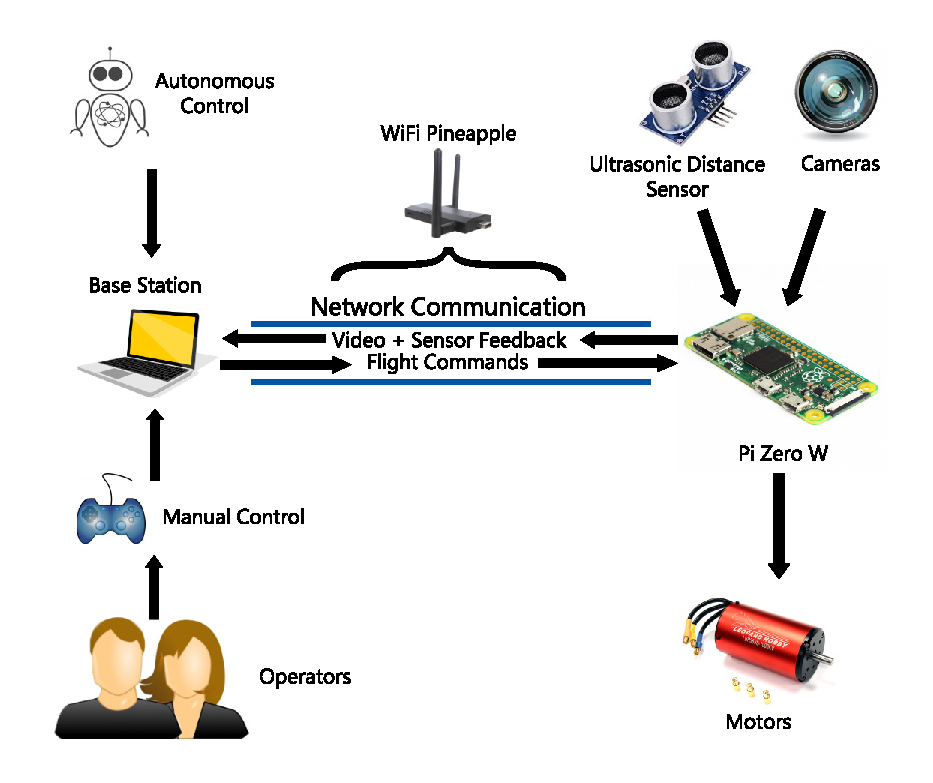
\includegraphics[height=3.5in]{DesignOverview}
\caption{Conceptual Design Overview}
\end{figure}


\subsubsection{Design Components}

\subsubsection{Device Communication} 

The communication between the aircraft and the base station will be connected by WiFi. Data is transferred over a 2.4GHz channel, allowing Raspberry Pi\cite{r3} board and base station to receive and transmit data when they are in the range of a WiFi network. We will establish a WiFi network by using a router, specifically the WiFi Pineapple\cite{r12}. In the event of communication loss, the vehicle should attempt to reconnect for no more than 3 seconds. If the connection is not re-established, the vehicle will shut down the motors. 


\subsubsection{Hardware}

The two main logic control components are the base station and the Raspberry Pi\cite{r3}. These two components will be able to communicate to each other through the WiFi Pineapple router\cite{r12}. The Base station will handle the difficult computations regarding image processing and flight planning. Additionally, the base station will be able to select between manual control mode or autonomous control mode using a GUI. The Raspberry Pi will handle motor control logic, and elevation control. Video and sensor information will be based from the Raspberry Pi to the base station, and directional commands will be returned from the base station to the Pi. 


\subsubsection{Flight Control}

We will connect motor controllers to the Raspberry Pi with GPIO pins. We will write a GPIO access program to access GPIO pins and establish communication with motors. We can configure the GPIO pins to start and shutdown the motors. Furthermore, we can set the logical voltages either low or high to change the speed. This code to control the motors will be able to handle commands from both manual and autonomous inputs.


\subsubsection{Sensors}% (camera + ultrasonic)

Camera Sensors are used to easily capture images. For the manual flight, the camera sensor will stream video (image frames) back to the base station. For the autonomous operation, these “images” can be used by video-processing algorithms for recognizing the target, searching the home-base, and operating the hover-hold. We will equip two cameras to our aircraft. One front Camera to process stream video and one at the bottom to find targets and the landing places.


The ultrasonic sensor can emit a specific frequency of sound waves and listen to that sound wave bounce back. The sensor can record the elapsed time between the sound wave being emitted and the sound wave bouncing back\cite{r11}. Once we know the speed of the sound wave, it is able to calculate the distance between the ultrasonic sensor and the object. we will use an ultrasonic sensor at the bottom of aircraft to detect the height from the ground and measure the boundary range.


\subsubsection{Image Processing}

All image processing will be done on the base station to increase calculation performance. Image processing should be able to distinguish four main objects: Delivery targets, packages, boundary lines, and obstacles. Once these objects are correctly identified, the autonomous system will then have to identify where that object is located in correlation to the vehicle. After a general location is established (Left, Right, in front, below, ect.) The autonomous system should then send the appropriate flight commands to the vehicle. 

\subsubsection{User Interface}

The user interface should be simple, with only the necessary information needed to control the micro air vehicle displayed. There should be a white button to enable manual flight control, as well as a red button to stop all flight commands. At minimum the front facing camera stream will be displayed on the user interface. The second camera stream may be added if computational power is not significantly compromised. Additionally, image processing overlays may also be added under the same circumstances. 



\subsection{Design Viewpoints} % (viewpoints are just an in-depth explanation of a certain aspect of the design)

\subsubsection{Introduction}  
	Viewpoints are an in-depth evaluation for each of our above design components. Here we will break each viewpoint into three primary categories: design concerns, design elements, and design examples. Design concerns address what we are trying to solve, and what problems we are anticipating to come across. Design elements will break down the specific goals of each viewpoint. Within the deign elements we will elaborate on each specific task and a general idea of how it will be implemented. In design examples we will review any existing technologies that might solve the viewpoint we are addressing. If there are no existing technologies, then we will review similar applications and explain what we are doing differently. 



\begin{center}
    \begin{tabular}{|c|p{0.3\linewidth}|p{0.4\linewidth}|}
        \hline
		Design viewpoint & Design concerns & Example Design Concepts \\
        \hline
		Communication & Reliability, Fail-safe Operations  & Video streaming applications and standard data packet transfer over WiFi.  \\
		\hline 
        Hardware & Reliable, Lightweight, Multi-functional & Raspberry pi, CSI cameras, Ultrasonic sensors, WiFi Pineapple\\
		\hline 
        Image Processing & Object Detection, Directional Translation & OpenCV, Matlab Image toolbox, directional markers  \\
		\hline 
        Flight Control & Motor control, Logic outline, Input Arguments  & ESC motor controller and GPIO pins.  \\
		\hline 
        Positioning & Ultrasonic Distance sensors, Image distance calculations  & OpenCV distance and positioning calculations, distance based on ultrasonic readings.  \\
		\hline 
        User control & User Interface, Manual Control Methods, Emergency Shutdown  &  Web interface attached to the base station system with basic user controls. \\
		\hline 
    \end{tabular}
\end{center}

    

\subsubsection{Communication Viewpoint} 
\begin{itemize}
 \item{ \textbf{Design Concerns:}}

The main design concern for communication is maintaining a low-latency, high-bandwidth connection between a base station and the vehicle. Design considerations should be made based on what will best address the above design constraint. Additional concerns about communication distance and strength will be secondary considerations for this project. \\ 

\item{ \textbf{Design Elements:}}

There are three objects that rely on steady communication channels: The base station, the vehicle, and the router. The router will act as an intermediary to the base station in order to boost the signal range, and produce a local network that the vehicle can connect to. The base station will connect to the router via USB or Ethernet cable, and the vehicle will connect over the 2.4GHz wireless channel. This creates a closed network that we can easily secure to communicate from our base station to our vehicle and back. Video and Ultrasonic Sensor information will be passed from the vehicle to the base station, and the flight calculations will be returned to the vehicle for execution. \\

\item{ \textbf{Design Examples:}}

Typically MAV's are controlled using radio communication, so our approach to this is not conventional. The main reason behind this is because WiFi has limited range compared to radio communication methods. For our application we will be in relatively close proximity to the vehicle, so this makes WiFi a better option for data throughput. \\


\end{itemize}



\subsubsection{Hardware Viewpoint} 
\begin{itemize}
\item{ \textbf{Design Concerns:}}

Our primary concerns with hardware is being lightweight enough to fit within the constraints of our vehicle requirements, and being able to communicate to the vehicle reliably. We will elaborate on our hardware decisions below based on those primary requirements. Secondary considerations will be based on ease of use, and project implementation. 

\item{ \textbf{Design Elements:}}
Our hardware requirements are limited to a couple different factors. The following components are needed for our implementation: A camera, a distance sensor, a base station, a router, and a vehicle controller. The vehicle controller is our most constrained object because it is limited by our size and weight limitations. This is why we decided to use the Raspberry pi zero. This computer is one of the most powerful computer for it's size on the market, and it is extremely inexpensive. Our camera was also decided base on this choice because is was specifically designed for the CSI input for the raspberry pi. The router (WiFi Pineapple) is based on what was on hand, but it also has the added benefit of not needing an external power source. The base station can be implemented on any laptop as long as it is capable of running Ubuntu or another Lunix distribution.  

\item{ \textbf{Design Examples:}} %If there are any!

Our design is typical of any server-client relationship. Our base station will act as the sever, while the vehicle is acting as the client. The client (vehicle) relays information from their data sources back to the server. The server will then perform the difficult computations that the client is not capable of handling. There is an intermediary, the router, which is also found in any client-server relationship. This element is less documented, but equally as critical to the overall success of the project.
\end{itemize}


\subsubsection{Image Processing Viewpoint}
\begin{itemize}
\item{ \textbf{Design Concerns:}}

The concerns of image processing can be separated into two parts: object detection and directional translation. During competition, the object to be detected is the envelop with two colors which are white and red. The envelop might not be in the original video range at the beginning of our flight, so the detection depends on the path of vehicle. During flight, the angle of the cameras will be changing. This causes the view of object to also change. Positions and shapes can increase the difficulty of detecting the object. The directional translation component is based on the relative location within the images received by the cameras. The view from cameras alone cannot estimate exact distances, so sensor and mathematic calculation based on known sizes can decrease the deviation. \\

\item{ \textbf{Design Elements:}}

At the start of the flight, the cameras will capture video. The video data will send to the base station via WiFi router. If the software cannot discover the object, then it will continue to move around the environment. If the object in the range of camera, base station will calculate a path to pick up the package. According to the path, the vehicle will convert this path into movements. On the way to pick up the object, the micro helicopter will avoid any obstacle it encounters. The base station will keep track of movements and make sure the micro helicopter arrives at the package pick up place. The micro helicopter will then pick up the envelop and attempt to bring it to the corresponding destination. \\ 
\item{ \textbf{Design Examples:}} %If there are any!

In order to process images, the vehicle needs a program that can handle streaming video in an efficient manner. OpenCV and Matlab Image toolbox can accomplish this task. However, OpenCV is an open source library, while Matlab is a licensed product (which is available to students for free). OpenCV is focuses more on the object detection so it is a better choice.\\
\end{itemize}



\subsubsection{Flight Control Viewpoint} %(how do we talk to the motors)
\begin{itemize}
\item{ \textbf{Design Concerns:}}

The main design concern for flight control is maintaining a stable connection between the Raspberry Pi with the multiple ESC motor controllers and motors. Additional concerns will be ESC motor controllers sending the correct pulsing signals to motors with the commands received from the users. \\
\item{ \textbf{Design Elements:}}

Flight control will be accomplished through connecting the ESC motor controllers with the Raspberry Pi through the GPIO pins\cite{r14}. Then, we will have each ESC motors controllers with each motor and with an extended power bank. We will write a GPIO access program to enable the GPIO pins to write outputs to the ESC motor controllers, then proceed to signal the motors. Once the connection completed, users can control the flight by sending the command to the Raspberry Pi board.\\

\item{ \textbf{Design Examples:}} %If there are any!

There are many examples of this using typical radio communications to control air vehicles. These are low-latency algorithms used to convert simple directional inputs into frequency based control algorithms for the ESC controllers. \\

\end{itemize}



\subsubsection{Positioning Viewpoint} %(distance + camera positioning)
\begin{itemize}
\item{ \textbf{Design Concerns:}}

The concern for positioning are the measurement accuracy of the ultrasonic sensor and the deviation between the realistic distance with the distance calculated by the image processing algorithm.

\item{ \textbf{Design Elements:}}

Camera sensors and ultrasonic sensors will be implemented to measure distance\cite{r15}. If we know the dimension of an object and we can use it as a reference to the image that collected by the camera sensor. Distance can be calculated with various of algorithms using OpenCV\cite{r13}. The ultrasonic sensor should be connected to the Raspberry Pi through the GPIO pins. Ultrasonic sensors can measure the distance to the ground by emitting specific frequency of sound waves and recording the elapsed time until sound wave bouncing back.

\item{ \textbf{Design Examples:}} %If there are any!

Distance from camera to object can be calculated through triangulation similarity. If we have an object with a known width W. We have initial distance from the object to the camera. Given the initial image collected by the camera sensor, we can measure the pixel width of the object in the image via OpenCV, marked as P. The focal F can be calculated as F = (P * D) / W. Then new distance D’ can be measured with the new pixel width in the later image. The formula will be D’ = (W * F) / P.\\
\end{itemize}



\subsubsection{User Control Viewpoint}% (how do we talk to the pi, talk about GUI)
\begin{itemize}
\item{ \textbf{Design Concerns:}}

The User interface should display 4 things. 2 video feeds, a manual override, and a emergency stop. The second window camera interface is completely optional because it is only needed for flight object recognition. The function buttons will take priority over the second window for a camera stream. \\
\item{ \textbf{Design Elements:}}

This is an interface required for the user to control the helicopter through the base station controller. The user will have control through an external controller for forward, backwards, up, down, left , and right. The user control interface also needs to be able to attached with web interface. \\ 
\item{ \textbf{Design Examples:}} %If there are any!

The physical controller can be na illustration for the user interface. Every controller should include all the basic functions needed, like turn left or right and move forward and backward. Our different directions should be represented by individual keys on the controller. And the emergency shutdown should be accessible through the controller or the user interface on the base station.
\end{itemize}


\subsection{Conclusion}

The Micro Air Vehicle challenge not only encompasses the design requirements listed above, but also the design requirements put forth by the Electrical and Mechanical sub-teams. While this design document provides a comprehensive coverage of the logical systems required, there are additional contributions that are not specified above. This document adequately outlines the design requirements for the Computer Science sub-team attached to Oregon State University's Micro Air Vehicle Challenge team. 




\newpage
	
\includegraphics[height=4cm]{coe_v_spot1}
        \hfill    
        \par\vspace{.5in}
        \begin{scshape}
        \centering
            \huge CS Capstone Technology Review \par
            {\large{Nov 20, 2017}}\par
            \vspace{8pt}
            \textbf{\Huge\CapstoneProjectName}\par
			\vspace{.5in}
                        {\large Prepared for}\par
            % \Huge \CapstoneSponsorCompany\par
            % \vspace{5pt}
            {\Large\NameSigPair{\CapstoneSponsorPerson}\par}
			\vspace{3pt}
            {\large Prepared by }\par
            \vspace{8pt}
            {\Large
                \NameSigPair{\GroupMemberOne}\par
                \NameSigPair{\GroupMemberTwo}\par
                \NameSigPair{\GroupMemberThree}\par
            }
            \vspace{.5in}
           \end{scshape}
        \begin{abstract}
        The purpose of this document is to evaluate technologies related to the implementation of our project. Our goal is to evaluate different technologies and determine the feasibility of each within the scope of our project. Each technology will be evaluated based on our selected criteria.  
        \end{abstract}   
        \normalsize

\newpage

\section{Technology Review}

\section*{Revision History}

\begin{center}
    \begin{tabular}{|c|c|c|c|}
        \hline
		Name & Date & Reason For Changes & Version\\
        \hline
		Technology Review & Nov 20, 2017 & Initial Creation & 1.0\\
	\hline 
    \end{tabular}
\end{center}


\subsection{Justin Sherburne's Role}

My role in the project as the computer science team lead is to effectively 
communicate project responsibilities and plans from the mechanical and electrical 
teams to my group. In addition to this I will also be developing the image 
recognition portion of our project. This will involve determining both hardware 
and software components of this implementation. The image recognition portion of 
our project will directly tie into our overall success in building an autonomous 
flying vehicle.  

\subsection{Hardware Controllers}

\subsubsection{Overview}

We were asked by the Electrical and Mechanical teams for this 
project to decide what hardware we would require on-board of our 
Micro-Air Vehicle. This is going to be the brains that directly 
interfaces with the motors. At minimum it should be able to 
translate manual commands into usable flight instructions for the 
vehicle. At most this hardware should be able to handle video and 
data streaming from a base station while maintaining a stable 
flight path. 

\subsubsection{Criteria}
\begin{enumerate}
\item{The controller should  be smaller than half of our maximum 
allowed dimension. This means it should be shorter than 8.85 inches 
in any dimension. However, smaller boards should be given 
preference in order to reduce our footprint on the overall design.}

\item{The controller should not use an excessive amount of power, 
and should not require an external power adapter. }

\item{The controller should have a port to attach to a camera. This 
can be USB, PCIe, CSI, I/O pins, ect.}

\item{The controller should have I/O pins capable of both 
transmitting and receiving electrical signals}

\item{The controller should be capable of maintaining a stable 
wireless connection via either built-in hardware or using an 
additional adapter.}
\end{enumerate}

\subsubsection{Potential Choices}

My initial research led me to two very similar options: The 
Raspberry Pi\cite{r3}, and the OpenRex. For a third option I am including 
the Arduino platform due to its versatility. Another possible third 
option I was considering was the Nvidia Jetson TX1. However, the 
Nvidia was the largest of the three options, and also required the 
most amount of power. 

\subsubsection{Arduino}


The Arduino platform is unique in the fact that it can be 
customized for most applications you could use a Pi or OpenRex on. 
Adding additional modules called shields to the base Arduino can 
give it wireless capabilities as well as USB and camera input 
options. Additionally, the MKR ZERO\cite{r24} is a similar size to the PiZero 
which makes it ideal for our application. Power is supplied via a 
micro-usb input, and runs on less than 2A. Additional boards may 
require separate power, however they can be powered in parallel 
with micro-usb adaptors with the same power supply. I/O pins would 
need to be utilized for additional shields added to the Arduino, 
however a specific shield could also be used for motor control. The 
Arduino has a micro-controller rather than a processor, meaning 
that it cannot support a true OS, and will generally be inferior at 
complex tasks. 


%https://store.arduino.cc/arduino-mkrzero

\subsubsection{Raspberry Pi Model 3}

The Raspberry Pi is one of the most commonly used controller boards 
because it is capable of running a full OS like Raspbian. It's 
power works identically to the Arduino platform, being supplied via 
micro-usb. In addition to being able to support an OS, the Pi also 
comes with additional ports built into the board. The CSI port is 
capable of handling a video feed from a camera, and USB ports can 
also accept camera inputs. There are two versions of the Pi that 
are suitable for our project; the Pi model 3\cite{r25}, and 
the Pi Zero W\cite{r3}. The Pi Zero is a smaller version of the 3, 
with less processing power, but still maintaining the on-board 
wireless capabilities. 
The processor is reduced on the Pi Zero, which is perhaps the 
largest difference between the two controllers. Both models also 
include 20 I/O pins that can be configured as needed. The Pi 3 
model B has 4 core processor running at 1.2GHz, however it only 
supports 1GB of ram. The Pi Zero has a single core processor 
running at 1GHz, in addition to 512MB of RAM.   


%https://www.raspberrypi.org/products/raspberry-pi-3-model-b/

%https://www.raspberrypi.org/products/raspberry-pi-zero-w/

\subsubsection{OpenRex}


The OpenRex\cite{r26} board is essentially a more-powerful version 
of the Pi 3. It includes a couple more ports like SATA as well as 
an on-board gyroscope. 
While some of these features could prove useful to the 
overall project, others are completely unnecessary for our 
application (like the humidity sensor). Additionally, the OpenRex 
does not have as much community support as the Pi and Arduino 
platforms. I/O, power, and size are nearly identical to the Pi, 
however, the OpenRex does not have built-in wireless communication. 
The OpenRex has a MX6 processor running 4 cores at 1.2GHz. 
Additionally, it supports up to 4GB of ram which means it could be 
capable of handling image processing without a base-station.  


%http://www.imx6rex.com/open-rex/

\subsubsection{Discussion}

The Pi is the strongest contender here for a number of reasons. The 
first being cost. While the Arduino is very comparable at \$35, the 
OpenRex board costs as much as \$335 for their top model. The Pi 
comes with a similar processor, and still includes a processor in 
its smaller form on the Pi Zero. The Pi Zero costs only \$10, and 
still includes the wireless capabilities that the Arduino and 
OpenRex do not have. The additional boards needed to run the 
Arduino and OpenRex add unnecessary complexity to the project. 

\subsubsection{Conclusion}

The Pi Zero W\cite{r3} is going to be our board of choice for this project. 
While it's processor is smaller than the Pi or OpenRex, our 
solution is to use the processing power of our base-station to our 
advantage. The small form factor reduces our weight and size while 
still keeping the camera, wireless, and I/O connections we need. In 
addition to being small, it is also the cheapest option and has a 
very large support community should we run into problems that are 
hardware specific. 



%%%%%%%%%%%%%%%%%%%%%%%%%%%%%%%%%%%%%%%%%%%%%%%%%%%%%%%%%%%%%%%%%%%%%


\subsection{Operating Systems}

\subsubsection{Overview}

For our project we will need 2 operating systems that are capable 
of interacting with each other in one form or another. One OS is for 
our controller on-board of the vehicle, and the second is for our 
base-station. In this comparison, all three OS's we are looking at 
are able to be implemented on either the base station or the Pi.  

\subsubsection{Criteria}

Operating systems will be evaluated based on the following criteria:
\begin{enumerate}
\item{The OS being loaded onto our controller must be lightweight 
and efficient, capable of running on a Pi Zero W}

\item{The OS running on our base-station must be capable of 
effectively utilizing the processing power of that system, in 
addition to being lightweight and stable.}

\item{Both operating systems should be based on a common platform 
and share similar file structures.}
\end{enumerate}

\subsubsection{Potential Choices}

There are quite a few Linux distributions floating around that 
could be very applicable to this project. However, Operating 
systems that are widely used will take precedence here because 
generally, they are stable over a variety of platforms. Because of 
this we will be looking into Raspbian for the Pi, as well as Win 10 
iot core. For the base-station we will be comparing Ubuntu to 
Windows architectures. It is important for these to be similar 
because it gives us flexibility during development. If we are 
running Windows we can develop an application on either device 
without needing to translate code for a different system.

\subsubsection{Rasbian}

Rasbian\cite{r27} is a Debian based operating system that is specifically 
designed for the Raspberry Pi boards. Since Pi's have been selected 
as our hardware of choice, it is a logical choice to use Raspbian as 
our default OS. The problem with Raspbian is that it is loaded with 
a lot of unnecessary programs that will not be needed for our 
project. The GUI is beneficial for troubleshooting, however it 
consumes resources and will ultimately be disabled to favor 
performance. 

% https://www.raspbian.org/RaspbianAbout

\subsubsection{Windows 10 / Win 10 iot Core}

Windows 10 and Win 10 iot core\cite{r28} are both based on the Windows 
architecture. The Win 10 core is capable of running on the Pi, and 
interfaces smoothly with other windows devices. Windows is stable 
and can effectively manage hardware resources for bulky programs. 
The downside to this is that there is a small community that is 
using the Win 10 core on the Pi, but support is limited. 
Additionally, if the Pi is not going to be running a Windows OS, 
then the base-station should be similarly converted. 

%https://developer.microsoft.com/en-us/windows/iot

\subsubsection{Ubuntu}

Ubuntu\cite{r29} is also Debian based, like Raspbian. This makes it a 
preferable choice over windows if the Pi is not running a Win 10 
iot core. Ubuntu is the most installed linux distro, and has a 
stable version available for free. There are also lightweight 
versions of Ubuntu, making it a possible candidate for running on 
the Pi as well. Ubuntu would allow us to easily communicate, 
develop, and test using one stable platform.  

%https://www.ubuntu.com/

\subsubsection{Discussion}

The key in this selection is finding a balance between two 
operating systems that results in simplicity. There are two clear 
options here. The first is a Windows 10 base-station combined with 
a Win 10 iot core running on the Pi. The second option is some sort 
of Debian - Debian configuration. This could mean Ubuntu to Ubuntu 
or Rasbian to Rasbian


\subsubsection{Conclusion}

It comes as little surprise that Raspbian is going to be the 
preferred OS for the Pi. It is lightweight enough to run 
efficiently on the Pi Zero, even with a GUI. The community support 
for Raspbian also gives it an edge over Win 10 iot core and Ubuntu. 
For our base station we should use Ubuntu, or a similar Debian 
based OS. Ubuntu is stable, widely supported, and can run alongside 
Windows on the same machine. Ubuntu will allow us to develop 
programs for the Pi without needing a special IDE. Additionally, 
using 3rd party utilities like OpenCV are simpler for Ubuntu / 
Raspbian because they are designed for a linux system.  





\subsection{Image Processing}

\subsubsection{Overview}

Our Micro-Air Vehicle is required to have an on-board camera system 
to stream video back to our base-station. So we are choosing to use 
this camera with an image-recognition software that is capable to 
finding the objects we need to look for during the competition. 
Image processing software is cumbersome, and with our Pi Zero we 
needed a unique solution to provide adequate processing power. So 
we are choosing to send the video feed back to our base station for 
processing, and sending the corresponding commands back to the 
controller. 

\subsubsection{Criteria}

\begin{enumerate}
\item{The program or software must be capable of running on a 
laptop that is not connected to the internet.}

\item{It must be able to identify the main obstacle located near 
the center of the competition area.}

\item{It must be able to identify the boundary lines that mark the 
edge of the competition area.}

\item{It must be capable of identifying landing areas, as well as 
the packages we need to pick up and deliver. }
\end{enumerate}

\subsubsection{Potential Choices}

Writing our own algorithm to locate objects is far beyond the scope 
of this project, so we need a third-party program for the base 
architecture. Matlab can be fairly lightweight if you do not 
include the GUI and additional packages, which makes it a viable 
option for this project. OpenCV and OpenSLAM are open source 
projects that could also meet our criteria. OpenCV is specifically 
designed for image processing, while OpenSLAM is intended for 3-D 
mapping projects. 

\subsubsection{Matlab - Image Processing Toolbox}

Matlab has many different packages that run with it. One of these 
packages is the Image Processing Toolbox\cite{r30}. This toolbox allows you to take a camera or video input and filter out colors, detect 
objects, and digitally stabilize video streams. The downside to 
Matlab is that it is bundled with other packages and isn't 
necessarily the most efficient processing option. For example, the 
image processing toolbox recommends being installed alongside six 
additional toolboxes. It does, however, run on a variety of 
platforms and languages making it simple to migrate from one device 
to another in the future. 

%https://www.mathworks.com/products/image.html

\subsubsection{OpenCV}

OpenCV\cite{r8} is an open source library the is designed specifically for 
computer vision and image processing. It runs in C, C++, Python, 
and Java. It also supports Windows, Linux, MacOS, iOS, and Android 
platforms. "OpenCV was designed for computational efficiency and 
with a strong focus on real-time applications. Written in optimized 
C/C++, the library can take advantage of multi-core processing." .
OpenCV is capable of filtering colors to identify specific objects. 
Additionally, by knowing a size of a specific object, OpenCV can 
then calculate its distance away from that object. 

%https://opencv.org/

\subsubsection{OpenSLAM}

SLAM stands for simultaneous localization and mapping. 
OpenSLAM\cite{r31} is an open-source repository of projects that 
utilize various SLAM algorithms to map environments. Essentially 
SLAM sets out to map a complete environment by tracking an objects 
location in approximation with a moving target. This requires an 
accurate measure of the vehicles speed, as well as a power computer 
to run the algorithm. While SLAM algorithms can be tailored to run 
on the available resources, it is primarily designed for 
applications like autonomous cars which can be fitted with powerful 
processing units. Additionally, it is intended to map 3 dimensional 
environments, not to filter for individual colors.

%http://openslam.org/

\subsubsection{Discussion}

Matlab provides a robust system that can also be used for other 
sensors and flight information. However, it is not the best option 
for image processing due to its required dependencies. OpenCV and 
OpenSLAM are both open source options that are fully capable of 
identifying the objects we need during the competition. OpenSLAM 
takes this a step further though and actively maps the environment 
we are flying in. 

\subsubsection{Conclusion}

OpenCV is going to be our preferred option here because it 
accomplished everything that the Matlab software can in a smaller 
package. OpenSLAM could be modified to locate colors during our 
competition, but the 3-D mapping functionality that it is intended 
for is not something we need to have for our project. OpenCV is the 
lightweight and simple option that accomplishes what we need it to 
do and nothing more. 


\subsection{Kaiyuan Fan's Role}
My role as a member of computer science team in this project is to actively share information with team leader and co-operate with the mechanical and electrical engineering teams. I will mainly work on implementing the autonomous flight of the vehicle.

\subsection{Data Collection Equipment}
\subsubsection{Overview}
We plan to design and manufacture a helicopter to participate in the 2018 micro air vehicle challenge competition. We are going to complete a delivery package mission in the competition. The delivery and pickups location areas are roughly known, the exact location of each area of interest is unknown and there has a rectangular obstacle between the base and the delivery area. Therefore, our flying vehicle needs to equip sensors to be able to find the targets, detect the obstacles, stay flight within the mission boundary and search the landing places.

\subsubsection{Criteria}
\begin{enumerate}
\item{The sensor should be able to collect data to measure the distance to the ground and the objects, the accuracy, and range of measurement should fit the competition environment.}
\item{The weight of sensor should be light enough to match the competition requirement.}
\item{Sensors should provide enough information for both manual fight and autonomous flight.}
\item{Sensors should be easy to find on market and should not be expensive.}
\end{enumerate}

\subsubsection{Potential Choices:}
The camera sensor is the most common choice for collecting images. By my research, there are various of sensors available on the market and I find the ultrasonic sensor and infrared sensor could be potential choices.

\subsubsection{Camera Sensor}
Camera Sensors can easily capture the images. For autonomous operation, these “images” can be used by video-processing algorithms for recognizing the target, searching the home-base, and operating the hover-hold. For the manual flight, the camera can collect the most significant real-time stream video and send back to the pilot.

\subsubsection{Ultrasonic sensor}
The ultrasonic sensor can emit a given frequency of sound waves and listens to that sound wave bounce back. The sensor can record the elapsed time between the sound wave being emitted and the sound wave bouncing back. Once we know the speed of the sound wave, it is able to calculate the distance between the ultrasonic sensor and the object. A minimum distance from the sensor is required to provide a time delay so that the “echoes” can be interpreted. \cite{r32} Ultrasonic sensor can measure distance without damage and are easy to use and reliable. 

\subsubsection{Infrared sensor}
Infrared sensors use infrared radiation to detect an object. "The main use of infrared sensors in robotics is for obstacle avoidance".\cite{r16} It also can use for measuring distance without touching a surface. Similar to the ultrasonic sensor, but two close infrared sensors measure distance by shining a beam of infrared light and uses a photo-transistor to measure the intensity of the light that bounces back. The response speed of infrared sensor can be fast but the range usually under 20 ft.

\subsubsection{Discussion}
Ultrasonic sensors can be used to control or indicate the position of targets and obstacles. Some objects might not be detected by ultrasonic sensors. This is because some objects are "shaped or positioned in such a way that the sound wave bounces off the object", but are deflected away from the Ultrasonic sensor. It is also possible for the object to be "too small to reflect enough of the sound wave back to the sensor to be detected"\cite{r11}. Ultrasonic sensors and infrared sensors can both be used to detect obstacles, but cannot easily to process data to make it suitable for visualization like the camera sensors. Infrared sensors have a relatively short distance measurement. All three types of sensors are cheap and can be easily found at the market, but the camera is the best technology to use for implementation. With the OpenCV support, we can detect the different targets and landing places with their colors. We can even measure the distance to the object if we know the original size of the object. The camera is the essential technology in our implementation.

\subsubsection{Conclusion}
We are going to implement two cameras in our design. One in front Camera to process stream video and one at the bottom to find targets and the landing places. We also decide to use an ultrasonic sensor at the bottom to detect the height from the ground and measure the boundary range. The helicopter can be stable hover at an altitude and accomplish various tasks with these two technologies.


\subsection{Video Stream Interface}
\subsubsection{Overview}
In this project, we are choosing Raspberry Pi as our helicopter’s board. Raspberry Pi is a powerful board, we are using Raspberry Pi Camera Module to collect and send stream video (image frames) to our base station. It’s necessary to receive the stable and reliable stream video from the helicopter, so the pilot can manual the flight. We need to use an interface to communicate between the camera module to the base station.

\subsubsection{Criteria}
\begin{enumerate}
\item{The video stream interface should stream video should under a reasonable latency.}
\item{The video stream interface should support the UDP (User Datagram Protocol) for data transmission.}
\item{The video stream interface should support the Raspberry Pi camera module and convey high-quality stream video.}
\end{enumerate}

\subsubsection{Potential Choices:}
We have been implemented the MJPG-streamer and it worked well. I found there are plenty of choices we can choose, I will discuss two common technologies: VLC media player and RPi-Cam-Web-Interface.

\subsubsection{VLC media player}
VLC media player (commonly known as VLC)\cite{r18} is a free, open-source, and cross-platform media player. VLC is available for desktop operating systems and mobile platforms, including the Raspberry Pi. It's easy to install the VLC media player on the Rasberry Pi board and use it to stream video to another device.

\subsubsection{ MJPG-streamer }
MJPG-streamer\cite{r20} is also a free and open-source interface. It uses command line application that copies JPEG frames from one or more input plugins to multiple output plugins. It can be used to stream JPEG files over an IP-based network from a webcam to various types of browsers and media players that are capable of receiving MJPG streams. It was originally written for embedded devices with very limited resources in terms of RAM and CPU.

\subsubsection{ RPi-Cam-Web-Interface}
RPi-Cam-Web-Interface\cite{r23} is a web interface especially for the Raspberry Pi camera module. It can be used for a wide variety of applications including surveillance and time-lapse photography. It is a free, open-source and highly configurable interface. It can be opened in any browser including the smart phones. The web interface includes motion detection, time-lapse, and video recording.

\subsubsection{Discussion}
All three interfaces support the user datagram protocol. In a real-time stream, some data loss may be acceptable with the aim of a timely display. VLC is easy to implement but have a relatively high latency compared to other applications. Both MJPG-streamer and RPi-Cam-Web-Interface can send reliable stream video to the base station. There are many other interfaces like pi-camera fits our video stream criteria. MJPG-streamer support various viewports. RPi-Cam-Web-Interface can extend to use motion detection and time-lapse photography.

\subsubsection{Conclusion}
We have various choices of the interface to stream video via the Raspberry Pi camera module. We will keep testing the best suitable one at the future time. Furthermore, we will be programming to implement OpenCV to detect the objects and measure distance in the streaming video.

\subsection{Communication}
\subsubsection{Overview}
Our helicopter need collect data and send to the ground station. The communication between helicopter and ground station should be reliable and stable. Communication requires high speed to process stream video, the communication latency and the connectable distance should be in a reasonable range.

\subsubsection{Criteria}
\begin{enumerate}
\item{The communication technology should maintain a transmit speed capable of two videos streaming at 720p 30fps. This is equivalent to roughly 15Mb/s.}
\item {The communication should be stable under the range of 40 ft.}
\item {The communication technology should follow the competition rule with the standard communication frequency 2.4 GHz.}
\end{enumerate}

\subsubsection{Potential Choices:}
Our flying vehicle needs be able to remotely communicate with the base station. Wireless communication technology is the prerequisite. The WiFi and Bluetooth are two effective wireless communication technology. While I only find these two technologies, I opened the scope of research and include wired ethernet as the potential choice.
\subsubsection{WiFi}
WiFi, or Wireless Fidelity\cite{r17} is the name of a popular wireless networking technology that uses radio waves to provide wireless high-speed Internet and network connections. WiFi technology are commonly using in our daily life. WiFi allows networking of computers and our flying vehicle without the need for wires. Data is transferred over radio waves, allowing WiFi capable devices to receive and transmit data when they are in the range of a WiFi network. 

\subsubsection{Bluetooth}
Bluetooth is another wireless communication technology. It is can exchange data over short distances by using radio waves at the 2.4GHz band. "By using the 2.4 GHz band, two Bluetooth devices each other can share up to 720 Kbps of capacity"\cite{r22}. The connectible range of Bluetooth is relatively low as 10 meters, about 30ft.

\subsubsection{Wired Ethernet}
Ethernet is a network technology commonly used in local area networks. "A wired Ethernet connection can theoretically offer up to 10 Gb/s"\cite{r21}, and the transmit speed is consistent. Wired networks are less expensive, faster, and more secure than wireless networks. However, the wired ethernet provides these advantages, it also has its biggest disadvantage, the immobility.

\subsubsection{Discussion}
Wired communication is incapable for our project while it provides the best transmit speed and stability. Our helicopter must use the wireless communication technology. The Bluetooth cannot give us enough transmit rate compare with the WiFi, the transmission rate can not able to support two videos streaming. The connectible distance of Bluetooth usually under 30ft. Our helicopter will travel and send data as far as 40ft, the connection will be unstable when the distance increases. WiFi can provide much more reliable and stable communication between the helicopter and the ground station. 

\subsubsection{Conclusion}
We are using Raspberry Pi Zero W which including the wireless network module and Bluetooth. WiFi is the best choice as our communication technology to send and receive data. The network will be provided by the competition area or by our own network router.



\subsection{Yingshi Huang's Role}

My role is to learn from requirements and help to design and calculate data in our sub-team. I will focus my efforts on controller integration and communication methods.

\subsection{Wireless Communication}
\subsubsection{Overview}

According to the requirements from the competition, either a remotely-controlled or full-autonomous system is needed. Regardless of our choice here, a wireless communication system will be required for the micro-helicopter. Wireless communication not only can connect with one devices; it is capable to connect with multiple devices at the same time.  Wireless communication is easy to access and convenient compared with other communications. In wireless communication, there are various choices like infrared communication, radio, blue-tooth, WiFi, mobile communication and so on.

\subsubsection{Criteria}
\begin{enumerate}
\item{Wireless communication will be the bridge to exchange data between the vehicle and computer.}
\item{Micro-helicopter will receive data from the wireless communication}
\item{Wireless communication will be able to receive data from vehicle}
\end{enumerate}

\subsubsection{Potential Choices}

My current knowledge gives me only two options blue-tooth and Wi-Fi. However, the choices two options are not enough, so my research has provided more options like infrared communication, radio, mobile communication.

\subsubsection{Infrared communication}

Infrared communication is a high-speed short range wireless communication\cite{r33}. It needs to transfer data directly from devices to devices, but does not use a traditional network. It is relatively inexpensive, and data will not lose easily. The communication range is ten to thirty meters. The speed of transferring data is fast, with a maximum speed of 100 Mbps. However, the communication can only control one device at a time. Obstacles like doors, walls, bad weather will affect the infrared communication. Infrared communication will also provide a strong power which can be harmful to human body.
%http://ieeexplore.ieee.org/document/554222/

\subsubsection{Bluetooth Radio}
Bluetooth\cite{r22} is another example of short range communication between devices. The range of transmission range is within 10 meter in common devices. The distance range can manage by the power of the senders and the receivers. Bluetooth system operates in unlicensed 2.4-GHz frequency. Nowadays, bluetooth is a common tool for transferring data. The normal rate of transmission is 1 Mbps. It is a tool which has replaced the use of infrared communication.

%wireless communication

\subsubsection{Mobile communication}
Cellular systems is the most common communications used by mobile cell. The mobile uses the signal from the signal towers. The area of the signal supply from the tower is like a cell. And there are many signal tower to combine as the whole system. Our team does not have rights to use the signal tower and the usage of the phone company can be expensive.

\subsubsection{WiFi communication}
WiFi is defined as an abbreviation for wireless fidelity. It is common to use for computer networking. If person has set up WiFi at a place, this person can access the computer network within a certain range of distance. The signal from the WiFi can get through the walls or doors, if they are made of woods. The WiFi communication can even send or receive signal from upstairs or downstairs. The WiFi communication can transmit data at 2.4 GHz frequency. The frequency of the communication can be change by devices. The average rate of transmission data is about 50 Mbps to 100 Mbps. It is easy to set up in a new place. 

\subsubsection{Discussion}
2.4-GHz frequency is recommended from the rules of the competition\cite{r2}. So that it becomes one of the reasons that the cellular system has been excluded from the other wireless communications. The second main reason for excluding the cellular system is the budget of using it. Image processing and video processing are operations which need high-speed data transmit tunnel. Infrared communication is not as fast as what operations are expected.

\subsubsection{Conclusion}
According to the previous consideration, WiFi and bluetooth are better choices than others communications. Both of the communication is easy to purchase on the market and have similar price. Compare with the transmission of the data, WiFi has a higher speed. As a result, WiFi becomes better choice of communications.

%%%%%%%%%%%%%%%%%%%%%%%%%%%%%%%%%%%%%%%%%%%%%%%%%%%%%%%%%%%%%%%%%%%%%
\subsection{Communication Protocol}

\subsubsection{Overview}
Communications between three hardware: micro-helicopter and base station, base station and remote controller.


\subsubsection{Criteria}
\begin{enumerate}
\item{Micro-helicopter will receive data from the base station and respond to movement.}
\item{base station will get information from the remote controller which provides data to the micro-helicopter for re-positioning.}
\end{enumerate}

\subsubsection{Potential Choices}
Based on our previous choice of WiFi for transmission method; UDP, TCP and Web-Internet will be considered as methods to connect hardwares.

\subsubsection{UDP}
UDP stands for User Datagram Protocol\cite{r35} and uses of data transferring. UDP will not acknowledge the receipt of the sending data. It means a disadvantage that no resends for lost data. On the contrary, an advantage is that save time without re-sending missing data. It is typical for immediate data such as online video, audio transmission, online gaming. Intermittent video or audio is an appearance of Lost data.

\subsubsection{TCP}
TCP stands for Transmission Control Protocol which is connection-oriented and re-transmittable. An advantage is able to resend data and acknowledge lost segments. A disadvantage is extending sending time. TCP is representative of sending guarantee data like Web-Page, files.

\subsubsection{Web-Internet}
Web-Internet is a tool using internet via the web to communicate. An advantage is that no need for storage in base station and able to calculate data on other devices. A disadvantage is that all data depend on transferring which requires unhindered signal transmissions.


\subsubsection{Discussion}
In theory, the computer will need lots of data to calculate distance and movement. Ensure data received is not as important as using data to calculate more rough distance, interrupted data is still value to estimate length and size of target and obstacles. Although 2.4GHz radio might be impacted, this communication is still able to send and receive data between woods and thin walls.

\subsubsection{Conclusion}
Due to the complexity of the systems being implemented on our project we will likely use a combination of these three technologies. Web-internet will be used for our GUI to interface with the vehicle. UDP will be used for the video-stream to the base-station, and TCP will be used as the transmission protocol between the base station and the vehicle. 


%%%%%%%%%%%%%%%%%%%%%%%%%%%%%%%%%%%%%%%%%%%%%%%%%%%%%%%%%%%%%%%%%%%%%
\subsection{Controller System}

\subsubsection{Overview}
Here I will be analyzing the link between the human giving the commands to remote controller and the reactions of vehicle. Possible remote controllers can be keyboard, a game-pad, and a radio control transmitter.

\subsubsection{Criteria}
\begin{enumerate}
\item{The remote controller can send the signals to micro-helicopter, and make the progressions of movements.}
\end{enumerate}

\subsubsection{Potential Choices}

\subsubsection{Keyboard}
Keyboard has more command keys available than the others. However, the joystick and radio control transmitter can also enough keys for our purposes. The advantage of the keyboard is that the keys are separated and precise. The disadvantage of that relationships is reactions and respond will slower be caused by pressing different keys.

\subsubsection{Joystick}
A Joystick is easy to learn how to use. However, it is hard to control the joystick with precisely. The advantage is less time of human reaction and easy use by different ranges of ages. The disadvantage is hard to control the micro-helicopter for small movements.

\subsubsection{Radio control transmitter}
Radio control transmitter is typical to use for micro-helicopter. Typically the manufacturers are selling micro-helicopter and radio control transmitters together. The advantage is a lower cost of material and higher profits. The disadvantage is larger and heavier.

\subsubsection{Discussion}
According to the requirement of movements of the micro-helicopter, the tunnel has enough space for movement and obstacle are able to avoid with a joystick. Too many connections are not accessible for the pilot to use in the tunnel which needs to avoid the obstacles and picking up target. Radio control transmitter has weaker signal and larger equipment.

\subsubsection{Conclusion}
Comparing the three possibilities; the keyboard has too many distractions. The Radio control transmitter will add too many weights for the micro-helicopter. So the better choice between increasing the weight and fewer distractions will be the joystick.

%%%%%%%%%%%%%%%%%%%%%%%%%%%%%%%%%%%%%%%%%%%%%%%%%%%%%%%%%%%%%%%%%%%%%
\subsection{Autonomous System Data}

\subsubsection{Overview}
Non-human control of micro-helicopter moving, pre-written code for distance calculations and exact movements depend on calculations.

\subsubsection{Criteria}
\begin{enumerate}
\item{Correct calculations from information}
\item{Using calculations to make movements}
\end{enumerate}

\subsubsection{Potential Choices}

\subsubsection{Data from sensor}
Distance sensor is a small tool to get a certain range of distances directly. The advantage to use distance sensor is receiving data directly and no need to wait calculations. The disadvantage for distance sensor is vibration of the micro-helicopter will affect the precision ratio of the distance. Incorrect distance might cause a crash to obstacle or unable to pick up the target which will lead to failure.

\subsubsection{Images from camera}
Cameras can provide more information than distance sensor. However, more data as input will need more calculation. More calculation will need correspond libraries. And it will need more time and energy to finish the tasks.

\subsubsection{Built-in Libraries}
Software libraries will help the computer calculate data. Most of the formula are provided in libraries which is used for calculate. However, it require more storage and computer burning. It is a factor to slow down the result of calculations.

\subsubsection{Acceleration Positioning}
It is a method for calculating from the target or obstacles to micro-helicopter. It need time for computer to process, but all information can be handle by computer it, which mean fewer energy waste.

\subsubsection{Discussion}
Distance will be a tool to help estimate the distance calculation but not providing correct information. Accelerate positioning depends on the images from cameras, but not necessary depend on the software libraries. However, software libraries can reduce the coding error.

\subsubsection{Conclusion}
It is better to have correct data than not allowable error data which can lead failure. So using a camera to receive and calculate data is better than receiving direct data from sensor.

\newpage

\section{Weekly Blog Summaries}
\subsection{Justin Sherburne}
\subsubsection{Fall 2017}
		\begin{description}
			\item{Week 1} - Set-up OneNote, and modify resume for submission.
			\item{Week 2} - Groups assigned, first meeting with project sponsor.
			\item{Week 3} - Tour of Columbia Helicopters, first group meeting.
            \item{Week 4} - Problem statement, initial project design and research.
			\item{Week 5} - Order initial equipment for CS, requirements document.
			\item{Week 6} - Begin setup of the Raspberry Pi Zero.
            \item{Week 7} - Technology Review document, Raspberry Pi streaming to laptop.
			\item{Week 8} - Technology Review, more video stream testing.
			\item{Week 9} - Thanksgiving week, no meetings or class. Revisiting old documents with new IEEE formatting. 
            \item{Week 10} - Design document, camera multiplexer arrived for testing.
		\end{description}
\subsubsection{Winter 2018}
		\begin{description}
			\item{Week 1} - Establish winter meeting times. 
			\item{Week 2} - OpenCV research, multiplexer testing, sponsor approval for modified documents.
			\item{Week 3} - OpenCV research on implementation, multiplexer found to be unusable.
            \item{Week 4} - OpenCV initial implementation on web-cam. Airframe is still being built.
			\item{Week 5} - OpenCV prototype for multiple colors. Motor and ultrasonic testing for the aircraft. 
			\item{Week 6} - Midterm report and poster rough draft due. March 16 deadline for limited autonomous function.
            \item{Week 7} - OpenCV tracking is finalized, begin work on Pi streaming into openCV.
			\item{Week 8} - Develop simple OpenCV GUI, including on-the-spot calibration. Streaming from the Pi to the Base station completed.
			\item{Week 9} - Beginning to adapt OpenCV to autonomous flight calculations. Helicopter is flying for the first time. 
            \item{Week 10} - Begin development of the Autonomous flight system. Aircraft motors are experiencing too much current and need replaced. AHS video of competition readiness. 
		\end{description}
\subsubsection{Spring 2018}
		\begin{description}
			\item{Week 1} - Autonomous flight progress. Meeting times established. New motors were delayed in shipping. 
			\item{Week 2} - Withdraw from AHS competition due to motor failure. Continue work on autonomous flight.
			\item{Week 3} - Autonomous corner detection is working. New motors have arrived and will begin installation. 
            \item{Week 4} - Autonomous controls output begins development. Final Expo poster submission. 
			\item{Week 5} - Modified corner detection for reliability. Autonomous controls established. Helicopter is being re-balanced after motor installation. 
			\item{Week 6} - Autonomous algorithm development. Flight testing with new motors. 
            \item{Week 7} - Finalize autonomous flight algorithms prior to code cut-off. Autonomous flight will not be tested on this airframe.
			\item{Week 8} - Expo.
			\item{Week 9} - Finalize documentation and project presentation. 
            \item{Week 10} - Finalize documentation and project presentation.
		\end{description}
        
        
\subsection{Kaiyuan Fan}
\subsubsection{Fall 2017}
		\begin{description}
			\item{Week 1} - Create OneNote structure, biography and handed in the resume.
			\item{Week 2} - Project was assigned, meet with the group mates and the sponsor.
			\item{Week 3} - Tour of Columbia Helicopters, start weekly meeting with TA.
            \item{Week 4} - Finish the Problem statement final draft and get verified e-mail.
			\item{Week 5} - Meeting with Anna from Columbia helicopter, talked about the funding and design change. 
			\item{Week 6} - Get approved of our problem statement and ordered equipment online.
            \item{Week 7} - Start working on the tech review and install OS for the Raspberry Pi.
			\item{Week 8} - Finished Tech review this week and implemented video stream on the Raspberry Pi board.
			\item{Week 9} - Thanksgiving week. Attend meeting with ME and EE team on Monday and submit the Tech review on November 21.
            \item{Week 10} - Finish the design document within the group and submit on Friday.
		\end{description}
\subsubsection{Winter 2018}
		\begin{description}
			\item{Week 1} - Establish winter meeting times.
			\item{Week 2} - First meeting with ME and EE team, discuss the project details.
			\item{Week 3} - Big group meeting talks about the team name, document due Jan 31st and equipment funding.		
            \item{Week 4} - Team name "Beaverhawk" was made.
			\item{Week 5} - Made decision on schedule of the competition. Start to work on the poster and demo.
			\item{Week 6} - Wired a DC motor on a breadboard with a power module and motor control board L293D.
            \item{Week 7} - Midterm report and presentation. Tested the change direction of DC motor by setting two GPIO pins output LOW and HIGH.
			\item{Week 8} - Made a template for motor control in CPP. Sent an intent of video delivery to Dr.Squires.
			\item{Week 9} - Did a feature on the user interface, read the user input by keyboard of HTML and pass the command to the Python script to control helicopter motors.
            \item{Week 10} - Build EE team motor control code in and add gamepad support to the remote web control system. Record the competition video.
		\end{description}
\subsubsection{Spring 2018}
		\begin{description}
			\item{Week 1} - Establish Spring meeting times. Expo registration.
			\item{Week 2} - Did not meet the bar for Gate 2 of the competition, project object change.
			\item{Week 3} - New motors are delivered and start the installation. 		
            \item{Week 4} - Added prevent key repeating feature in manual flight code. Tested keyboard event code on Windows. 
			\item{Week 5} - Added set motor servo back after turning feature in manual flight code. 
			\item{Week 6} - Submitted midterm progress report and the presentation. Code freeze on Friday.
            \item{Week 7} - Tested flight with new motors, have slipping shaft problem. Expo on Friday.
			\item{Week 8} - Expo has done.
			\item{Week 9} - Finalize documentation and project presentation.
            \item{Week 10} - Finalize documentation and project presentation.
		\end{description}


\subsection{Yingshi Huang}
\subsubsection{Fall 2017}
		\begin{description}
			\item{Week 1} - Read the project and follow OneNote pattern, put biography in file
			\item{Week 2} - Project assigned by instructor
			\item{Week 3} - Weekly meeting and tour
            \item{Week 4} - Problem statement and signature
			\item{Week 5} - Sponsor, funding and budget 
			\item{Week 6} - Research and order equipment
            \item{Week 7} - set up equipment and started gitHub
			\item{Week 8} - Tech review document and camera 
			\item{Week 9} - Big group meeting 
            \item{Week 10} - Submit document and Term review
		\end{description}
\subsubsection{Winter 2018}
		\begin{description}
			\item{Week 1} - Set up meeting time as early as possible
			\item{Week 2} - First detail meeting with ME and EE members
			\item{Week 3} - Team name and flyer
            \item{Week 4} - Testing and flying, competition readiness video is closing
			\item{Week 5} - Every member works on competition readiness video
			\item{Week 6} - EE team works on equipments connection
            \item{Week 7} - Midterm report and presentation
			\item{Week 8} - Joystick testing
			\item{Week 9} - Second week of joystick testing
            \item{Week 10} - Final report and presentation and Whole team final report
		\end{description}
\subsubsection{Spring 2018}
		\begin{description}
			\item{Week 1} - Review last team work and set up meeting with ME team and EE team
			\item{Week 2} - Due to late equipments delivery, cancel enter competition 
			\item{Week 3} - Two language communication found by python extension library 			
            \item{Week 4} - Build up environment of simple statement exchange 
			\item{Week 5} - Second test of new helicopter
			\item{Week 6} - Motor test
            \item{Week 7} - switch assignment from language to autonomous
			\item{Week 8} - Expo. GitHub filled.
			\item{Week 9} - Documation and presentation.
            \item{Week 10} - Documation and presentation
		\end{description}
        
\newpage
\section{Final Poster}
\begin{figure}[ht]
\centering
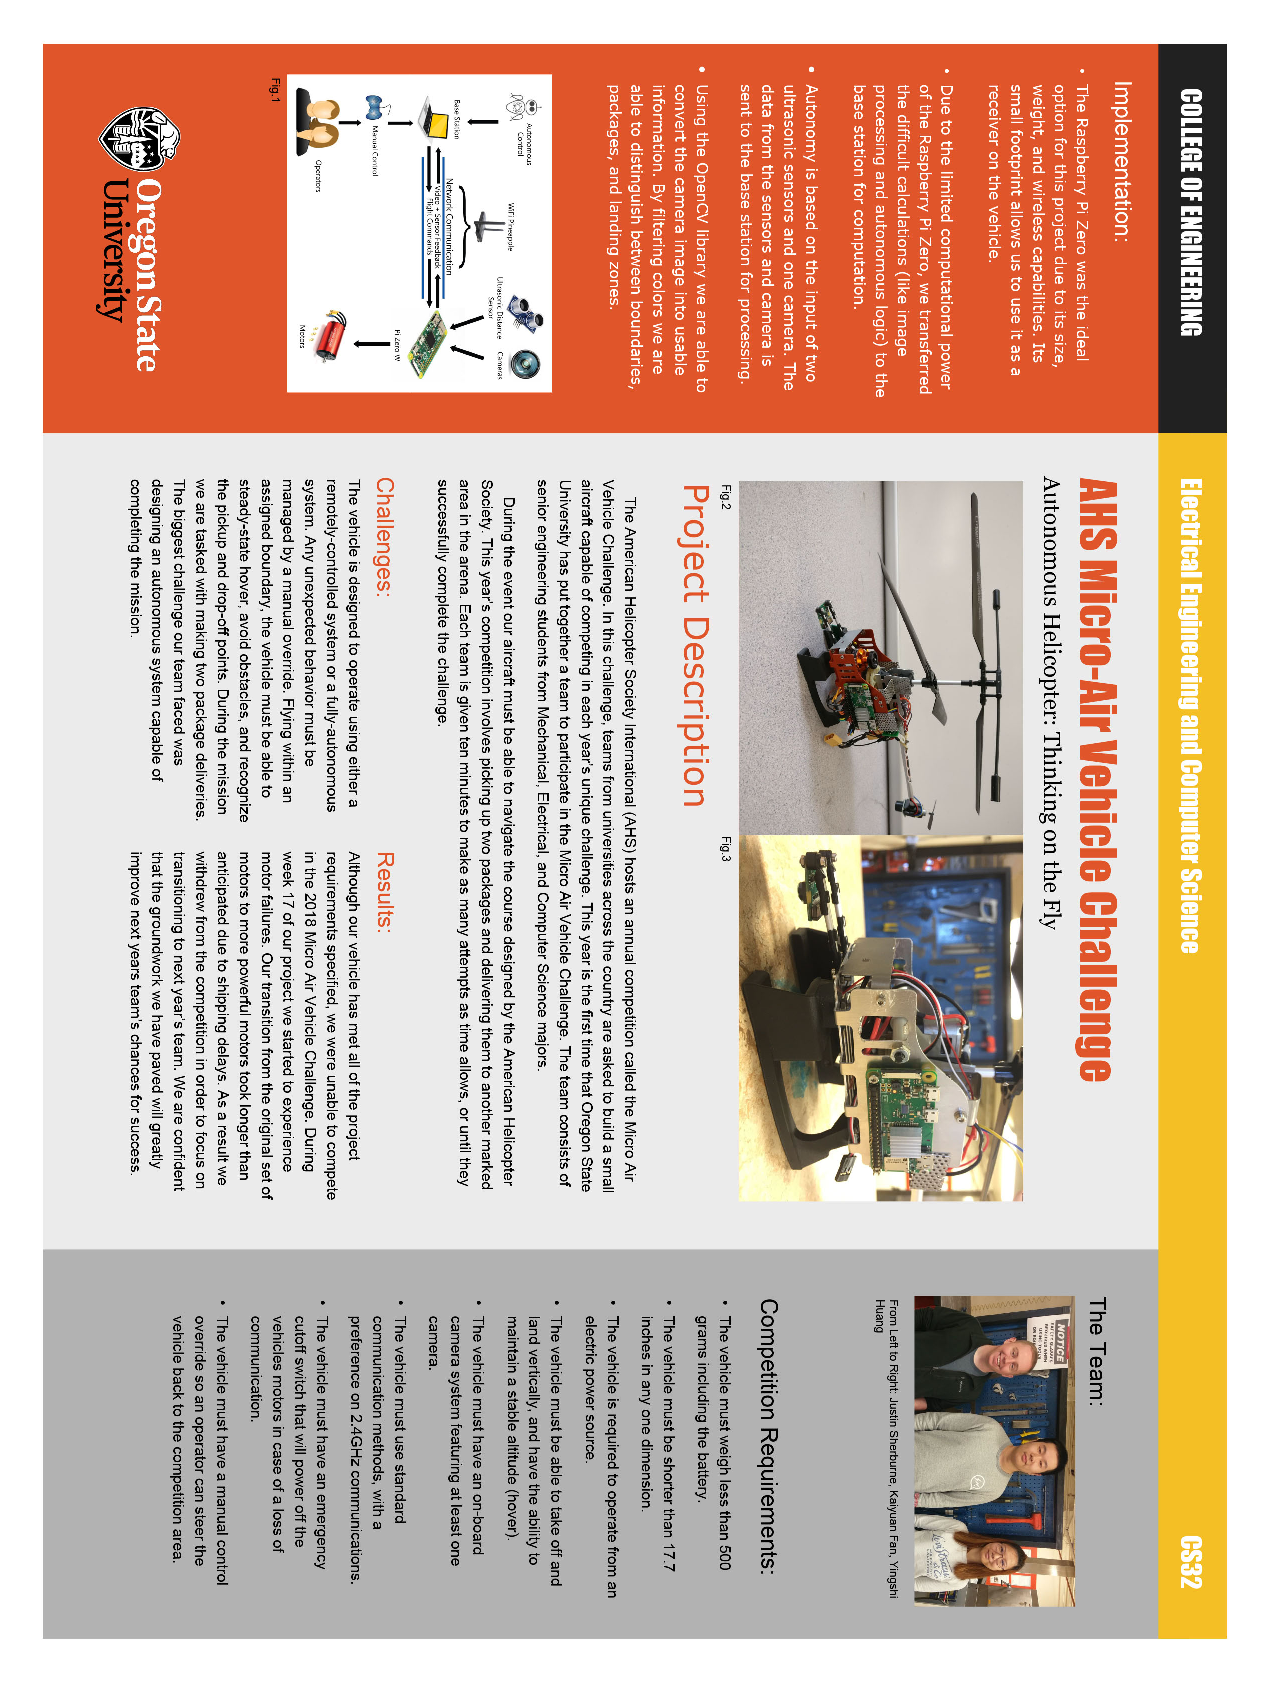
\includegraphics[height=7.5in]{poster_expo}
\caption{Expo Poster, Final Draft}
\end{figure}


\newpage
\section{Project Documentation}

\subsection{Project Design}

\begin{figure}[ht]
\centering
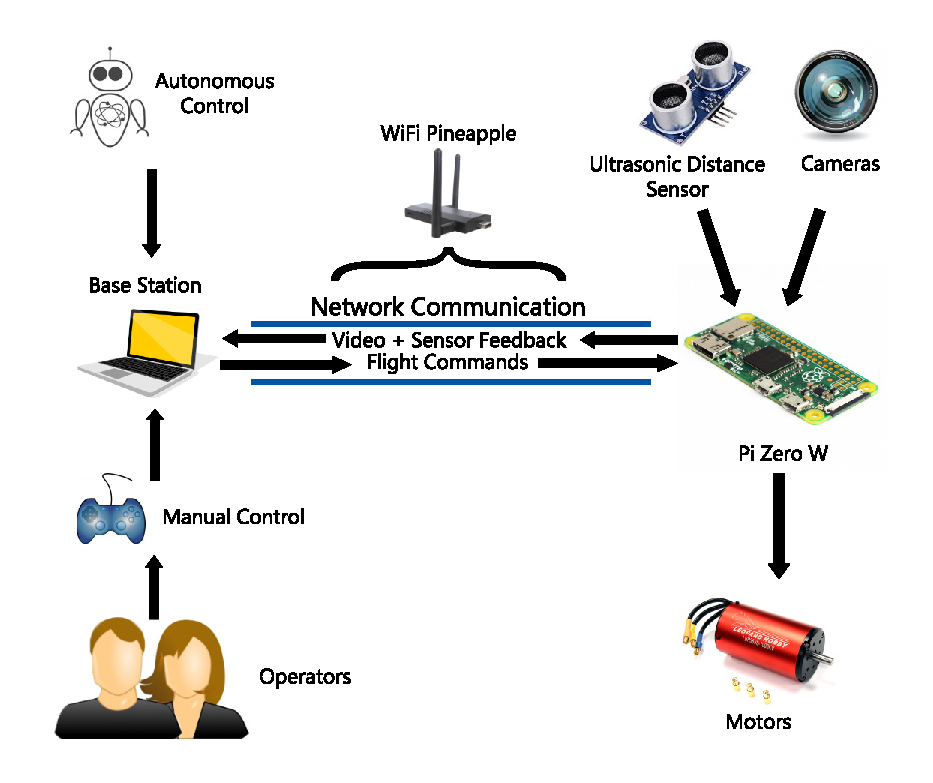
\includegraphics[height=3.5in]{DesignOverview}
\caption{Conceptual Design Overview}
\end{figure}

For our design we have two distinct systems: The Base Station, and the Raspberry Pi Zero. The Base Station controls the autonomous flight systems, serves as the link for manual control, hosts the GUI, and also runs the image processing system. The Raspberry Pi is the brains of the aircraft; operating the motors, ultrasonic sensors, and streaming the video feed back to the Base Station. These two systems are connected over a standard WiFi connection which can be set up a number of different ways. In our testing we used a device called a WiFi Pineapple, which acts as a short-range, compact wireless router. Above in Figure 3 you can see the overall architecture of our project.


\subsection{Software Installation}

In this section we will elaborate on how to install and use the software we have developed for this project. We will break the software into two components: The Base Station and the Raspberry Pi. While both devices are used together in this project, the software installation is not the same due to computational limitations on the Raspberry Pi. 

\subsubsection{Base Station Software}

To begin, the base station is simply a computer running a Linux-based operating system. In our case we used a laptop, but a desktop with a monitor could also be used if more processing power is required. The operating system we chose (and that these instructions will be based upon) is Ubuntu. Ubuntu is one of the most supported Linux operating systems, making is ideal for our project. Instructions and additional documentation can be found at https://www.ubuntu.com/. 

Once you are running your Linux distro, you will need to install OpenCV. OpenCV is the framework used for the image processing application, and will occupy nearly 2gb of hard drive space. The installation is fairly complex and may require additional troubleshooting outside of the scope of this document. For detailed installation instructions I would recommend following this guide: https://www.learnopencv.com/install-opencv3-on-ubuntu/ . This step may take up to 20 minutes. To verify that OpenCV has installed correctly I would recommend running some of the included samples or to try our image recognition program directly. 

Xdotool is required for the autonomous flight output. It is a Linux-only library and will not work on Windows or OSX. There is a similar library in Windows called Windows.h, however that library is incompatible with Linux. To install Xdotool, simply run: \texttt{sudo apt-get install xdotool} in the terminal. Additional resources for Xdotool can be found here: http://xmodulo.com/simulate-key-press-mouse-movement-linux.html .

Lastly, you will need a different web browser than Firefox. The GUI API does not work correctly with the Firefox web browser that is built-in to Ubuntu. Instead we used the Chromium web browser which can be installed via the Ubuntu Software center. 

The code developed for this project is located on our git-hub repository: https://github.com/OSU-Capstone-MAV-Challenge/CS\_MAV\_Challenge. This can be cloned to a directory using the following command:
\newline

\texttt{git clone https://github.com/OSU-Capstone-MAV-Challenge/CS\_MAV\_Challenge} 

\vspace{0.2in}
You will find the required software for the Base Station in /SourceCode/Base Station/. 

\subsubsection{Raspberry Pi Software}

On the Raspberry Pi we installed Rasbian OS. This is a lightweight version of Linux specifically designed for the Raspberry Pi. It includes native support for all of the Raspberry Pi Zero hardware. Installation instructions can be found here: https://www.raspberrypi.org/documentation/installation/installing-images/README.md . Once installed, it is recommended to remove any large libraries not being used in this project like Math-lab, and Wolfram Alpha. Removing these libraries, in addition to a high-speed SD card will drastically improve startup time. 

The following packages will need to be installed on the Raspberry Pi Zero:
\begin{description}
\item{PHP 7.0 \& Apache2} - Should come pre-installed, follow the following link for additional support: https://www.stewright.me/2016/03/turn-raspberry-pi-3-php-7-powered-web-server/
\item{Tornado Web Framework} - Installation instructions: http://www.tornadoweb.org/en/stable/
\item{RPIO} - Setup Instructions: https://pythonhosted.org/RPIO/
\item{mjpg streamer} - Documentation found: http://sourceforge.net/projects/mjpg-streamer/ or in our git-hub repository.
\end{description}

You will also need to clone the project's git-hub repository onto the Raspberry Pi. We will be accessing the files located under /SourceCode/RaspberryPi/.This can be done using the following command: 
\newline

\texttt{git clone https://github.com/OSU-Capstone-MAV-Challenge/CS\_MAV\_Challenge} 

\vspace{0.2in}

\subsection{Software Initialization}

While both systems must be powered on and connected to a local area network, the Raspberry Pi Zero must be configured first. During testing the Raspberry Pi can be initialized through a local terminal and the GUI if connected to an external display. This method will reduce performance, and should be avoided. Instead the configuration will be done through a SSH connection from the base station to the Raspberry Pi. In the future a script could be developed to run at startup to initialize these systems without needing to SSH to the Raspberry Pi.

\subsubsection{Raspberry Pi Zero}

To initialize the manual flight system, connect Raspberry PI and laptop in a same local area network. SSH into the Raspberry Pi using Putty or a terminal connection. Navigate to the correct subdirectory in the github repository and type \texttt{sudo python MotorControl.py}. This initialized the motor control server. To initialize the video streaming server navigate to /SourceCode/RaspberryPi/Streamer/mjpg-streamer/mjpg-streamer-experimental/. In this directory run the startup script to initialize the stream: \texttt{startup.sh}.


\subsubsection{Base Station}

The Index.html file contains the GUI for controlling the aircraft. This can be used with either keyboard input, an Xbox controller, or by manually clicking each button on screen. Simply right-click and open with your desired web-browser. 


To run the image processing software, navigate to /SourceCode/Base Station/OpenCV/. Here you can type \texttt{make} to compile the program, and \texttt{Vision} to run. On line 843 of \texttt{main.cpp} there are some toggles to turn on and off various features prior to compiling the program. 
\begin{description}
\item{\textbf{calibrationMode}} - Enables you to reset individual color settings on-the-go. Leaving it enabled with display the trackbars for re-calibrating colors and the filtered video feed; disabling it will hide both of those screens. This feature can also be toggled off at runtime using the Hide Calibration slider.
\item{\textbf{webcammode}} - Enabled allows you to use your built-in web-cam for troubleshooting. Rather than needing to connect to a remote camera, it will default to your web-cam video feed. Disabling this will prompt you to connect to a remote camera. In our case this will be the Raspberry Pi. If the video streaming software is already running, you only need to type the IP address of the Raspberry Pi, or the host name of the device.
\item{\textbf{threadded}} - true enables the autonomous flight calculations and commands, false disables the autonomous flight functionality. Autonomous calculations can also be stopped after the program has been started by using the autonomous slider in the main video window. 
\end{description}

Once the image processing software is running you can click back to the GUI and the autonomous commands will output directly to the web-page. To exit you must type \texttt{CTRL+C} to the terminal, or toggle the track-bar labeled kill. To switch to manual flight controls toggle the track-bar labeled autonomous.



\section{Team Retrospective}
\subsection{Justin Sherburne}

\subsubsection{Technical Information Learned} 
During the course of this project I learned a lot about the OpenCV library. It is a powerful tool for image processing applications, but can be just as difficult to learn as a new programming language. While I would have enjoyed diving a little deeper into OpenCV systems, there is simply too many features to try and learn in a term or a year. In addition to OpenCV I also learned about autonomous flight algorithms. While I was developing the flight system for our helicopter I quickly realized how complex an autonomous system really is. On paper it seems simple; given a specific input, output a direction of movement. In practice there are so many outside factors that you have to try and account for that make it non-trivial. Given autonomous vehicles only have to worry about two dimensions of travel, I grossly underestimated the complexity of this portion of the project.

\subsubsection{Non-technical Information Learned} 
I learned a lot this year about team management and communication. Our team faced many obstacles from both outside and inside sources. Being in an interdisciplinary project has given me great experience in project management. In addition to mt experience in the team, I also learned a great deal about project documentation. Using OneNote was a great way to stay organized and place all of my thoughts and research into one location. 

\subsubsection{Experiences: Project Work}
The amount of documentation that went into this project was unexpected. While I understand the need for elaborate planning for major undertakings like these projects, I believe there are certain parts that are unnecessary.There is quite a bit of redundancy in each document that covers aspects that have already been addressed. Additionally, I do not believe the technology review was adequate research for the project. Personally I spent several hours researching OpenCV and image processing technologies for our project, but my technology review did not reflect that accurately. Instead wrote 2 pages on operating system options, something that is a relatively trivial choice for our application. 

\subsubsection{Experiences: Project Management}
Project management was arguably the most important part of this project, and also one area we struggled with. Having an interdisciplinary project means there needs to be a steady stream of communication between all members of the group. For our team we used Facebook as our primary method of communicating, but not everyone checked our page each week. Posts would occasionally go unnoticed or ignored. A better method for communicating would have been google hangouts, a group text, or even some combination of e-mail and Facebook.

\subsubsection{Experiences: Teamwork}
Teamwork is another area that our team struggled with this year. A significant portion of this project fell heavily on one or two members of this team at a time, and work was never evenly distributed. I think part of the issue stems from not having clearly defined roles for each team member, and a lack of time management. During the course of this project we acted as individuals contributing to a common goal rather than a team. This means that large portions of the project or documentation were left to an individual as the rest of the team viewed that section as their responsibility or area of expertise.  

\subsubsection{Things to do differently:}
From a non-technical perspective, communication. Many of our problems could have been mitigated with clear communication from start to finish. Defining clear roles for each member is beneficial, but ideally any member should be able to take over development of any section at any point in time. Staying up-to-date with project progress is critical for the success of a team, and I think it also helps motivate each member. Knowing that your teammate is working and actively contributing to your project is an effective motivator for many teams. Communication allows you to keep your teammates up to date or to clue someone in that there is a meeting on Monday morning.

From a technical perspective we could have improved in many areas. Ideally, our image recognition software should be identifying shapes and features using machine learning, or object recognition rather than color. Our autonomous flight algorithm also could have used 2-3 more weeks of development with actual flight testing. One problem that plagued our group was our use of three separate languages in our project. Trying to get all three to work effectively together significantly impacted development. Lastly, knowing how the project progressed this year I would have placed more pressure on the Mechanical Engineering team to finish development. The Computer Science component of this project is the last to be implemented, and on both major deadlines we were given the aircraft with only a week to troubleshoot and get our systems running. 


\subsection{Kaiyuan Fan}
\subsubsection{Technical Information Learned}
The main technical information I have learned is using a microcomputer board to deliver a practical product. I learned programming on Raspberry Pi to host a web server and browser the webpage remotely to access the Raspberry Pi GPIOs. Through the previous nine months, I have learned to establish a webpage with an open source web framework to communicate with the script on Pi. I have learned to use AJAX to reduce the traffic travels between the client and the server, and I learned using the API in HTML which I have never been used before. In addition, I have learned how to interface different programming languages.

\subsubsection{Non-technical Information Learned}
The non-technical information I have learned is how to effectively do the research of the unfamiliar topics and properly communicate with the supervisors and my peers. Besides, I have learned to make OneNote blogs to keep track of working logs, and I also got benefits from making various documents.

\subsubsection{Experiences: Project Work}
The whole project is a long getting new problem and finding solution path. For this challenging project, we start with empty and have overcome many obstacles. We were facing trouble interfacing different programming languages. we got motor issues and there are problems occurred during the flight test. What I have learned is to solve the problems with the knowledge I have and the resources I can find.

\subsubsection{Experiences: Project Management}
We have our weekly meeting to keep track of the progress of the project. Each of us has the different focus on developing the project, we managed in this way to make steady progress.

\subsubsection{Experiences: Teamwork}
Through the three terms, we were collaborating with two electrical and three mechanical engineering members. We have set up weekly big group meetings and our CS sub-team meetings. Working in a team helps me learn. Our project is multi-disciplinary, so teamwork performed a significant role in our project. ME team worked on manufacturing and balancing the vehicle, EE team worked on the wiring and motor control script, and our CS team was implementing the autonomous and manual flight systems. We have encountered hardware delay problem by other teams, our CS team could not have sufficient time to test our implementation. We decided to do as much as possible before the hardware available. What I have learned is when we have negative factors within the team, each member should try their best to reduce the negative impact.

\subsubsection{Things to do differently:}
If I could do it all over, I would be more proactive. I would communicate more often with each other, so we could come out a testable aircraft sooner. I also would like to work on the image recognition portion since I hardly touch this part. In addition, I would like to deliver a more beautiful GUI and add the onboard camera streaming feed into it.

\subsection{Yingshi Huang}
\subsubsection{Technical Information Learned}
I have learned using different computer languages which are python and c++ to receive data from a joystick. I have also learned to how to control the pin on the raspberry pi w zero. And I believe raspberry pi is similar to many on market bands like banana pie and so on. The hardest part I learned from the last few terms is to connect two different computer languages. To send data from python to c can use by python extension library. It is an enrichment library, and you can learn a lot from this library. There is much information in it. I will continue to learn from python extension library.

\subsubsection{Non-technical Information Learned}
I have learned how to use LaTex and shared documentation with others. I also learn how to read lengthy technical documentation and technology guide. Not only learn how to read them I have learned how to write the technical review, verify email, and much other documentation. Not only skills related to academic but also communication and noting ability.

\subsubsection{Experiences: Project Work}
In the project everyone needs to understand not every part of the plans will fit the procession. In work, the project might be getting into some unexpected, and the problems cannot solve in a long time. It is a reason for the whole team to understand and find another way to cross the obstacles. If the team only have one plan, it is possible to face failure. The project is better to have a second plan and able to extra time to solve unexpected problems.

\subsubsection{Experiences: Project Management}
Our team did not have proper management, so a lot of works did not have enough time to finish. Excellent project management can help the whole group to work on the project and with better quality. All the assignments must complete by submit date, and each person is better to hand in the job early.

\subsubsection{Experiences: Teamwork}
For good teamwork, it is crucial to communicate smoothly with other members. Not only talk with your teammates in a right emotion but also make sure your teammate can understand what is your expression otherwise it is a wordless communication. And if your team want to finish the project in a better way, it is good to assign tasks to each member so that people can work on different parts and the project complete by the whole group on time.

\subsubsection{Things to do differently:}
Do more research before work on the project. The reason to do more research is that I had worked on the project but there is another more straightforward way to figure out the problem, but I missed it. According to the mistake, I understand that do more research can help yourself to know more detail and solve problems faster. Ask for more information from the instructor, be brave to talk with someone who had learned more from me. 


\section{Appendix A: Essential Code Listings}

\subsection{Team Git-hub Repository:}

https://github.com/OSU-Capstone-MAV-Challenge/CS\_MAV\_Challenge

\subsection{Kyle Hounslow's OpenCV tutorials:}

\textbf{Video Part 1:} https://youtu.be/RS\_uQGOQIdg

\textbf{Video Part 2:} https://youtu.be/ASCi7J5W1FM

\textbf{Video Part 3:} https://youtu.be/4KYlHgQQAts

\textbf{Part 3 Code:}

https://www.dropbox.com/s/o22cnih7v0mu7gv/multipleObjectTracking.cpp?dl=0

https://www.dropbox.com/s/rck1v0gjv0y1thy/Fruit.h?dl=0

https://www.dropbox.com/s/2bvdrcnlno878s8/Fruit.cpp?dl=0

\subsection{Raspberry Pi Resources:}

\textbf{Rasbian} - https://www.raspberrypi.org/documentation/installation/installing-images/README.md-

\textbf{PHP 7.0 \& Apache2} - https://www.stewright.me/2016/03/turn-raspberry-pi-3-php-7-powered-web-server/

\textbf{Tornado Web Framework} - http://www.tornadoweb.org/en/stable/

\textbf{RPIO} - https://pythonhosted.org/RPIO/

\textbf{mjpg streamer} - http://sourceforge.net/projects/mjpg-streamer/ or in our git-hub repository.

\subsection{Base Station Resources:}

\textbf{OpenCV} - https://www.learnopencv.com/install-opencv3-on-ubuntu/

\textbf{Ubuntu - }https://www.ubuntu.com/

\textbf{Xdotool} - http://xmodulo.com/simulate-key-press-mouse-movement-linux.html


\newpage
\bibliographystyle{IEEEtran}
\bibliography{references}


\end{document}
